\documentclass[titlepage]{article}
\usepackage[utf8]{inputenc}
\usepackage[english]{babel}
\usepackage{multirow}
\usepackage{float}
\usepackage{graphicx}
\usepackage{listings}
\usepackage{xcolor}
\usepackage{fancyhdr}
\usepackage{hyperref}
\usepackage{tabularx}
\newcolumntype{C}{>{\centering\arraybackslash}X}
\usepackage{booktabs}
\usepackage{adjustbox}


\graphicspath{ {./img/} }

\pagestyle{fancy}
\fancyhf{}
\lhead{}
\chead{}
\rhead{\leftmark}
\lfoot{}
\cfoot{\thepage}
\rfoot{}
\renewcommand{\headrulewidth}{0pt}
\renewcommand{\lstlistingname}{Codice}

\DeclareFixedFont{\ttb}{T1}{txtt}{bx}{n}{9}
\DeclareFixedFont{\ttm}{T1}{txtt}{m}{n}{9}
\definecolor{deepblue}{rgb}{0,0,0.5}
\definecolor{deepred}{rgb}{0.6,0,0}
\definecolor{deepgreen}{rgb}{0,0.5,0}

\newcommand\pythonstyle{\lstset{
  language=Python,
  backgroundcolor=\color{white},
  basicstyle=\ttm,
  otherkeywords={self},
  keywordstyle=\ttb\color{deepblue},
  emph={MyClass,__init__},
  emphstyle=\ttb\color{deepred},
  stringstyle=\color{deepgreen},
  commentstyle=\color{red},
  frame=tb,
  showstringspaces=false,
  numbers=left,
  stepnumber=1,
  showstringspaces=false,
  tabsize=1,
  breaklines=true,
  breakatwhitespace=false,
}}

\lstnewenvironment{python}[1][]
{
\pythonstyle
\lstset{#1}
}
{}

\definecolor{mygreen}{rgb}{0,0.6,0}
\definecolor{mygray}{rgb}{0.5,0.5,0.5}
\definecolor{mymauve}{rgb}{0.58,0,0.82}
\definecolor{terminalbgcolor}{HTML}{330033}
\definecolor{terminalrulecolor}{HTML}{000099}
\newcommand{\lstconsolestyle}{
\lstset{
	backgroundcolor=\color{terminalbgcolor},
	basicstyle=\color{white}\fontfamily{fvm}\footnotesize\selectfont,
	breakatwhitespace=false,  
	breaklines=true,
	captionpos=b,
	commentstyle=\color{mygreen},
	deletekeywords={...},
	escapeinside={\%*}{*)},
	extendedchars=true,
	frame=single,
	keepspaces=true,
	keywordstyle=\color{blue},
	%language=none,
	morekeywords={*,...},
	numbers=none,
	numbersep=5pt,
  framerule=2pt,
	numberstyle=\color{mygray}\tiny\selectfont,
	rulecolor=\color{terminalrulecolor},
	showspaces=false,
	showstringspaces=false,
	showtabs=false,
	stepnumber=2,
	stringstyle=\color{mymauve},
	tabsize=2
}
}

\definecolor{delim}{RGB}{20,105,176}
\definecolor{numb}{RGB}{106, 109, 32}
\definecolor{string}{rgb}{0.64,0.08,0.08}

\lstdefinelanguage{json}{
    numbers=left,
    numberstyle=\small,
    frame=single,
    rulecolor=\color{black},
    showspaces=false,
    showtabs=false,
    breaklines=true,
    postbreak=\raisebox{0ex}[0ex][0ex]{\ensuremath{\color{gray}\hookrightarrow\space}},
    breakatwhitespace=true,
    basicstyle=\ttfamily\small,
    upquote=true,
    morestring=[b]",
    stringstyle=\color{string},
    literate=
     *{0}{{{\color{numb}0}}}{1}
      {1}{{{\color{numb}1}}}{1}
      {2}{{{\color{numb}2}}}{1}
      {3}{{{\color{numb}3}}}{1}
      {4}{{{\color{numb}4}}}{1}
      {5}{{{\color{numb}5}}}{1}
      {6}{{{\color{numb}6}}}{1}
      {7}{{{\color{numb}7}}}{1}
      {8}{{{\color{numb}8}}}{1}
      {9}{{{\color{numb}9}}}{1}
      {\{}{{{\color{delim}{\{}}}}{1}
      {\}}{{{\color{delim}{\}}}}}{1}
      {[}{{{\color{delim}{[}}}}{1}
      {]}{{{\color{delim}{]}}}}{1},
}

\title{Application of the ant colony algorithm for a truck delivery distributed system}
\author{Fabrizio Corriera}
\date{30/11/2023}

\begin{document}

\maketitle

\pagenumbering{roman}
\tableofcontents
\newpage
\pagenumbering{arabic}

\section{Introduction}
In this work we explore the application of the ant colony algorithm to propose a vehicle routing model based on a dynamic pick-up and delivery problem (DPDP) inside of a distributed system.

The premise of this work is an experimentation about the application of a routing algorithm based on a heuristic model.

A heuristic model is a problem-solving or decision-making approach that relies on practical rules, intuition, and experience rather than strictly adhering to an optimal algorithmic solution. Heuristic models are employed when finding an exact solution is computationally expensive or impractical. Instead of exhaustively exploring all possible solutions, heuristics aim to quickly identify a satisfactory solution.

In the context of routing algorithms, heuristics play a crucial role in optimizing the pathfinding process. Routing algorithms determine the most efficient path from a source to a destination in a network or graph. Heuristic models in routing algorithms prioritize speed and practicality over guaranteeing the absolute shortest path. The purpose is to rapidly find a reasonably good solution without the need for exhaustive computation, which is particularly important in real-time applications.

The idea behind using heuristics in routing algorithms is to strike a balance between efficiency and accuracy. By leveraging informed estimates and rules of thumb, heuristic models can significantly reduce the computational overhead associated with finding optimal routes, making them well-suited for dynamic and resource-constrained environments. While the solutions provided by heuristic models may not always be optimal, they often offer a satisfactory trade-off between computational complexity and solution quality, making them practical for a wide range of applications.

\section{Functional requirements}
The project functional requirements are:
\begin{itemize}
    \item The main routing algorithm of the system must be a heuristic algorithm.
    \item The heuristic algorithm must be able to find a path for the vehicle in a reasonable amount of time.
    \item The tests must be run keeping in mind a real world scenario.
    \item The system is composed by many nodes that correspond to the vehicles.
\end{itemize}

\section{Tools used}
The tools used in this project are:
\begin{itemize}
    \item \textbf{Python:} Python is a high-level, interpreted programming language known for its simplicity and readability. It emphasizes code readability and allows developers to express concepts in fewer lines of code.
    \item \textbf{Ant colony algorithm:} The ant colony optimization algorithm is a nature-inspired optimization technique that mimics the foraging behavior of ants. It involves a population of artificial ants exploring and marking paths with pheromones to find the optimal solution to a given problem. The algorithm utilizes the principle of collective intelligence and pheromone-based communication to iteratively converge towards an efficient solution.
    \item \textbf{Open Street Map:} OpenStreetMap (OSM) is a collaborative, open-source mapping platform that allows users to create, edit, and share geographic data globally. It provides a free and editable map of the world, relying on contributions from a diverse community of mappers. OSM is widely used for applications such as navigation, geolocation, and urban planning.
    \item \textbf{OSMnx:} OSMnx is a Python package built on top of NetworkX and GeoPandas, and interacts with OpenStreetMap APIs that allows us to download and model street networks or other infrastructure anywhere in the world with geospatial features.
    \item \textbf{JSON:} JSON (JavaScript Object Notation) is a lightweight data interchange format that is easy for humans to read and write and easy for machines to parse and generate. It uses key-value pairs and supports nested structures, providing a widely adopted standard for data exchange between web servers and clients.
\end{itemize}

\section{Project structure}
During the designing phase of the project we try to work keeping in mind a few key concepts:
\begin{itemize}
    \item Modularity: we want to develop this project in a way that we can easily modify it or add features with relative ease.
    \item Efficiency: knowing that this application should run on mobile devices, we try to develop a code that keeps computational costs at minimum.
    \item Decentralization: as far as possible we try to keep this system as decentralized as possible, minimizing failure points and keeping communications between devices as light as possible.
\end{itemize}
So, we will present the project structure keeping in mind two different representations:
\begin{enumerate}
    \item The \textbf{Vehicle} as its own environment.
    \item The vehicle as a node in the \textbf{Network}.
\end{enumerate}
\subsection{The vehicle}
The vehicle in this project is represented as the set of all its properties, specifically:
\begin{itemize}
    \item Position
    \item Storage
    \item Energy
    \item Scheduled path
\end{itemize}

So, we create the \textbf{Truck} class for keeping track of all these internal variables regarding the vehicle status.

From this point on we start implementing in the class some methods that will be useful in the general schema of the project: mainly we focus on the path of the vehicle, expanding it in many ways, until we realize that we need dedicated data structures for it, and that's why we proceed to implement new classes for the management of the vehicle path.

Then another interesting consideration was how to deal with the algorithms and computations involving how to find the ideal path for the vehicle. Considering that these kind of computations would require the management of a lot of resources not directly related to the vehicle itself, we decided to implement another class for the pathfinding.

\subsection{Route management}
During the development of the project we realize the need for a class, or more classes, that might help us with the management of the vehicle's path. These classes must answer to these needs:
\begin{itemize}
    \item We need a class that helps us abstract the route list of the vehicle.
    \item The route list must be sort of a middle point between human representation and easy to compute data.
    \item We need to micromanage different aspects of this data structure.
    \item We must also think of a way to make the possible communication of this data easy.
\end{itemize}

From all these considerations we realized that what we needed was to create a hierarchical structure of classes:

\begin{itemize}
    \item \textbf{RouteList}: This is the object with which the vehicle class interacts directly, using its methods and its structure to interact and manage the list of stops that are scheduled.
    \begin{itemize}
        \item \textbf{Job}: This is kind of a middle object, the one containing information about a full job (withdrawal+delivery). This object is useful mainly for communication between nodes and server, giving us a useful and common way to communicate new jobs.
        \begin{itemize}
            \item \textbf{Stop}: Stop is the brick class, basically a RouteList is a list of Stop objects, with some high level methods that allow us to manage the sigle stops inside of it. The Stop object should be very transparent, and almost invisible to the other classes, allowing to deal with it just through the RouteList object.
        \end{itemize}
    \end{itemize}
\end{itemize}

\subsection{Pathfinding}
For all the pathfinding related issues we implemented a class called RouteCalculator, that, from the road graph of the town, and the access to the Truck object can do all the computations we need for solving the already mentioned pathfinding related problems.

The 3 key features we want to implement are:
\begin{enumerate}
    \item Resolving the smaller pathfinding problems related to the paths from point to point.
    \item Being able to compute the ant colony algorithm locally.
    \item Using a greedy algorithm to compute the smaller deviations to add new nodes in an already existing path.
\end{enumerate}

So, the way we imagined this class is using certain methods to obtain the information regarding the city streets, their length, their speed limits and average speeds and travel times, and then we use those information as support to the two main computation algorithms (greedy algorithm and ant colony algorithm), this way we don't need to know about the complexity of every computation behind it.

\subsection{Networking}
The networking design for this project is very simple; considering the following principles:
\begin{itemize}
    \item We want our system to be as decentralized as possible
    \item We still need a central point to dispatch requests
    \item We want the system to be able to work in case of failure of any $n-1$ nodes
    \item We want to minimize clients-server communication
\end{itemize}

A \textbf{P2P network} with a slightly modified \textbf{discovery server} seems like the optimal solution.

The nodes will communicate with the server just when joining the network (during initialization), obtaining the list of already connected nodes, and then they will be able to communicate with each other.

The server will not be a pure discovery server, as intended in a normal P2P network, but it will also be able to send job requests to the nodes (in broadcast). Since we want to minimize server-nodes traffic, we will let the nodes decide in that case which node will take the job and then just contact the server to inform it of the decision.

\section{Development}
We will now show the code implementation for the project as we described it in the previous section. We will explain the code and our design choices class by class:
\begin{enumerate}
    \item Stop (plus StopEncoder and StopDecoder)
    \item Job (plus JobEncoder and JobDecoder)
    \item RouteList
    \item Truck
    \item RoutesCalculator
    \item Plotter
    \item Node
    \item Server
\end{enumerate}

\subsection{Stop}
\begin{figure}[H]
    \centering
    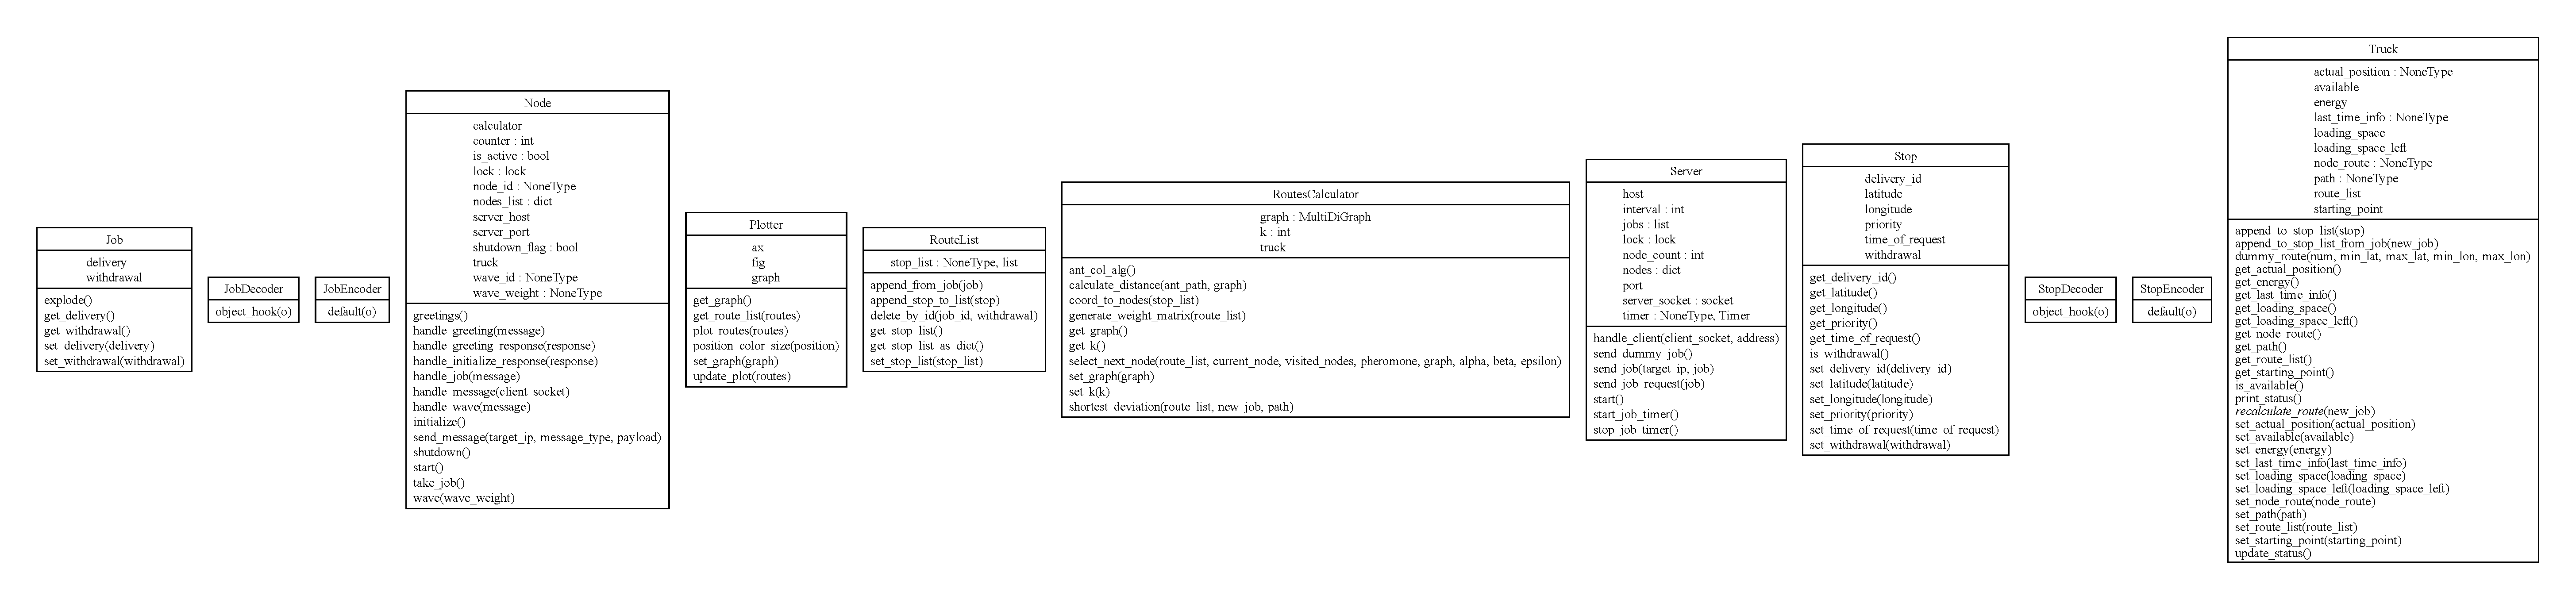
\includegraphics[trim={68.5cm 5cm 21.3cm 5cm}, clip, scale=.5]{img/classes.pdf}
    \caption{Attributes and methods of the Stop class}
    \label{fig:stop_class}
\end{figure}

\begin{itemize}
    \item \textbf{delivery\_id}: This is a unique value used to identify the correlation between a withdrawal and a delivery.
    \item \textbf{latitude}: Geographic coordinate for the stop relative to the distance form the equator.
    \item \textbf{longitude}: Geographic coordinate for the stop relative to the distance form the reference meridian.
    \item \textbf{priority}: A numerical value that gives us the priority of the stop (default=1, high priority$>$1, low priority $\in [0,1[$).
    \item \textbf{time\_of\_request}: This datetime variable gives us the time at which the request was forwarded (this might be useful in order to boost the priority of old requests).
    \item \textbf{withdrawal}: Boolean flag value that informs us if the stop is actually a withdrawal (True) or a delivery (False).
\end{itemize}

The methods for this class are just setters and getters of the above mentioned attributes. Basically this class is our data structure for all the useful informations regarding the  stops.

\subsection{Job}
\begin{figure}[H]
    \centering
    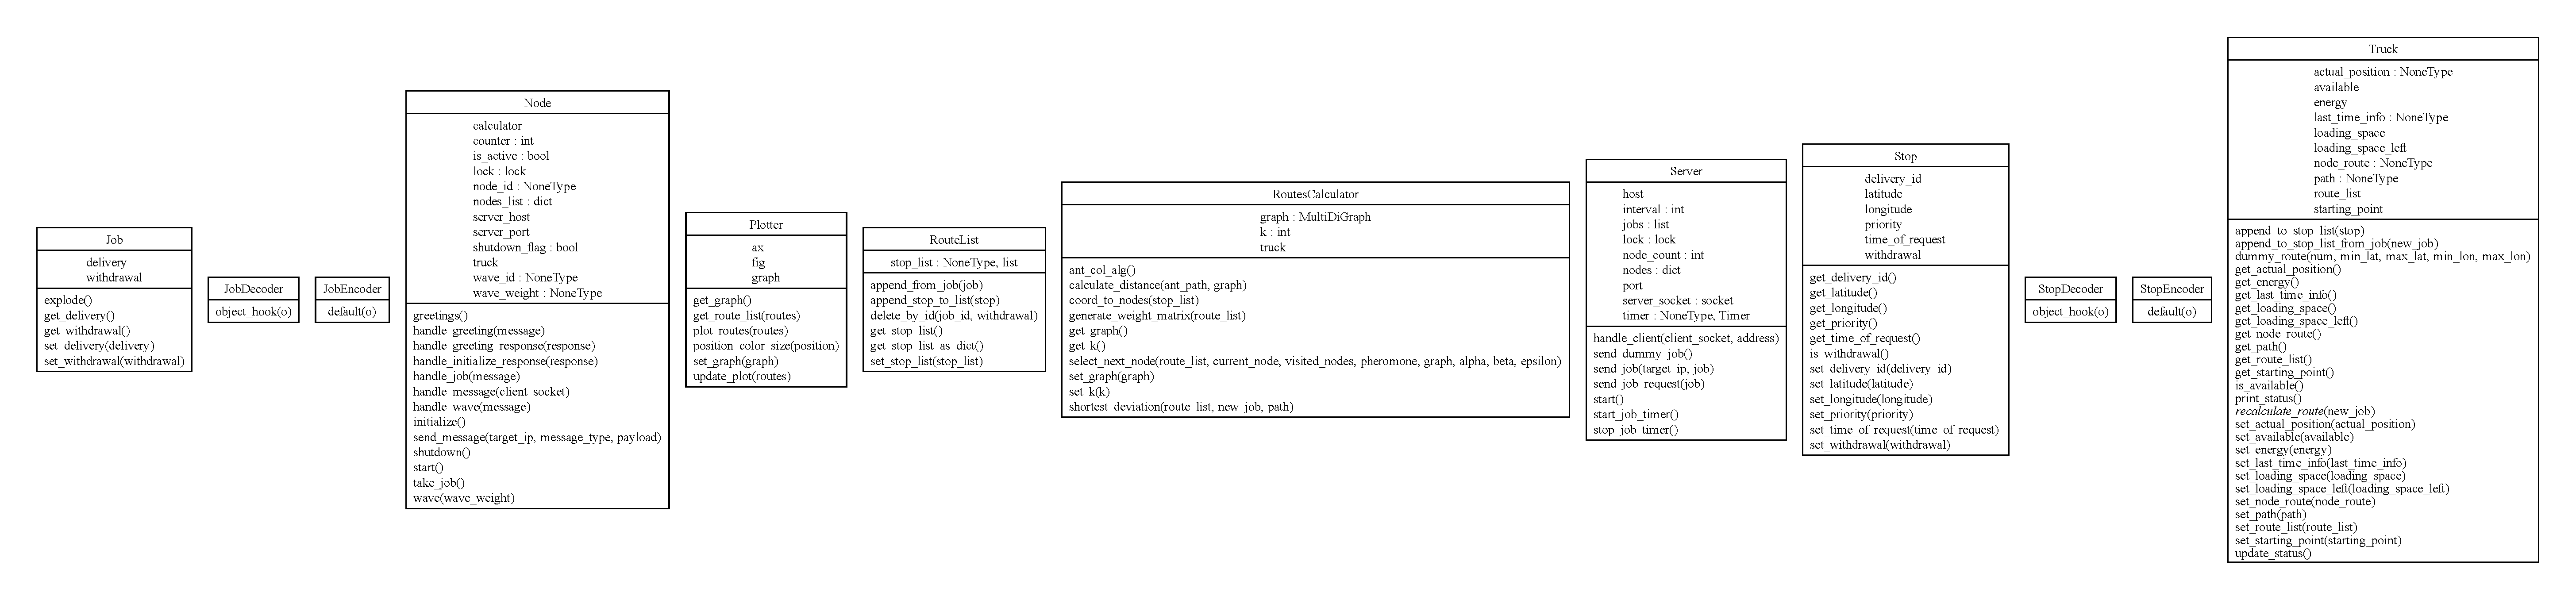
\includegraphics[trim={0 8cm 91cm 8cm}, clip, scale=.5]{img/classes.pdf}
    \caption{Attributes and methods of the Job class}
    \label{fig:job_class}
\end{figure}

\begin{itemize}
    \item \textbf{delivery}: The stop object containing information about the withdrawal operation of this job.
    \item \textbf{withdrawal}: The stop object containing information about the delivery operation of this job.
\end{itemize}

This class exist mainly as a tool for communication between server and nodes (when the server has to inform the nodes of a new job request). One main drawback regarding this implementation may be about the use of just one withdrawal object and one delivery object, but actually the code is implemented in a way that we could easily adapt this class using more than one delivery (or even more than one withdrawal); it could be easily adapted.

The only method worth mentioning is \textbf{explode}, that just returns the single stops.

\subsection{RouteList}
\begin{figure}[H]
    \centering
    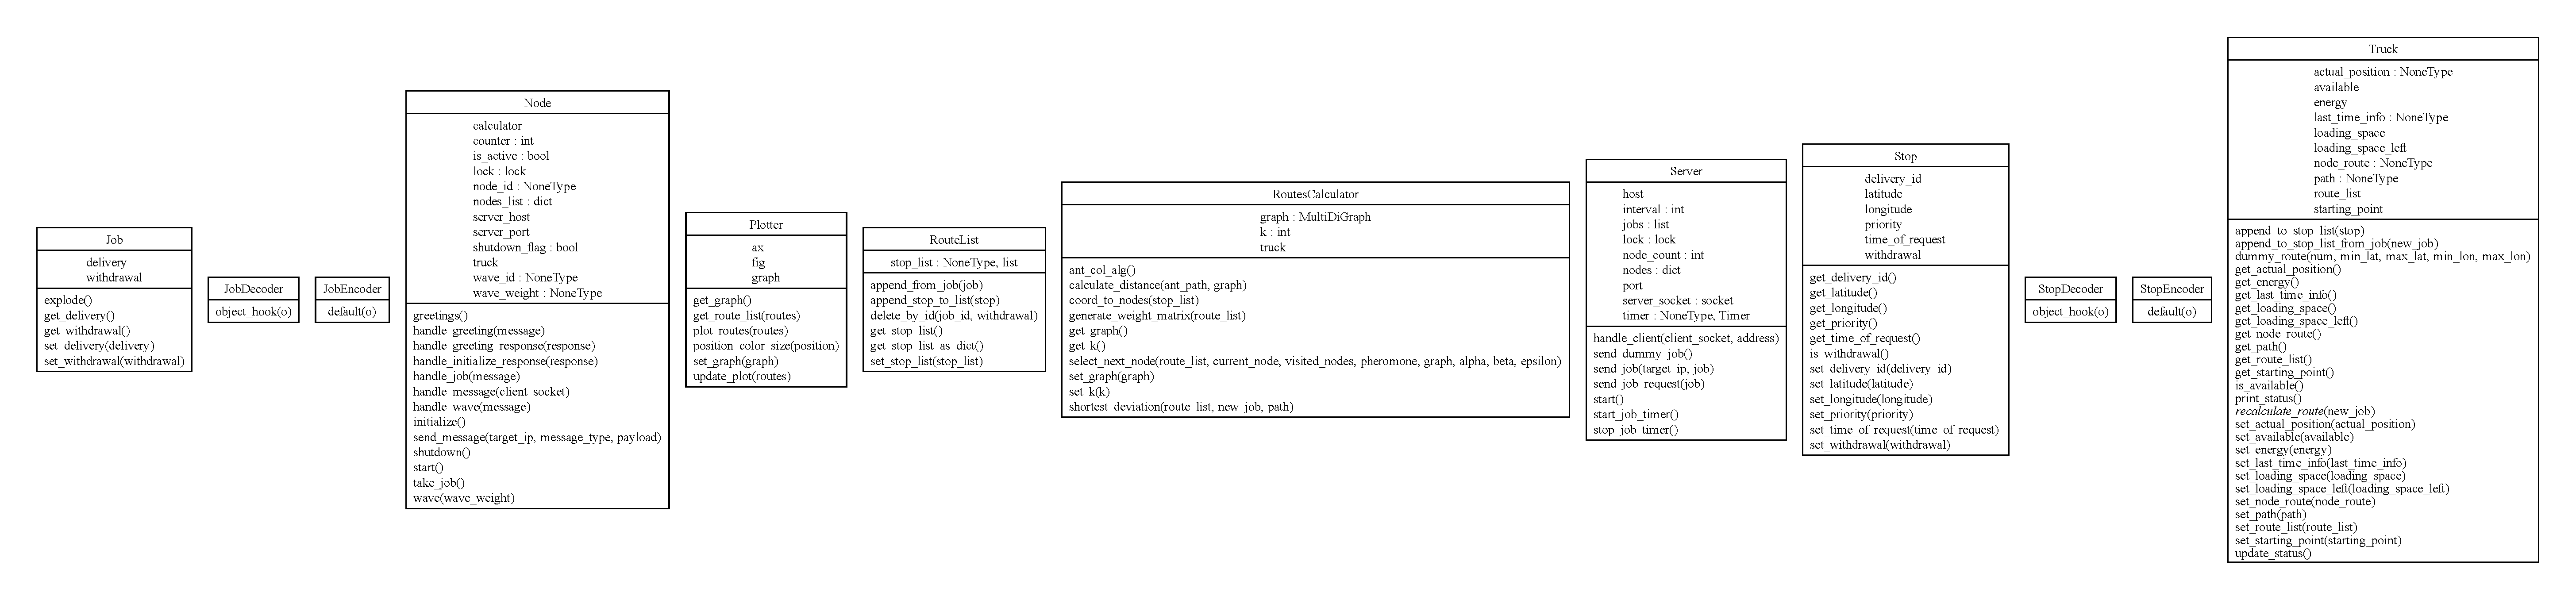
\includegraphics[trim={33cm 8cm 58cm 8cm}, clip, scale=.5]{img/classes.pdf}
    \caption{Attributes and methods of the RouteList class}
    \label{fig:routelist_class}
\end{figure}

\begin{itemize}
    \item \textbf{stop\_list}: This is a list object containing multiple Stop objects.
\end{itemize}

Though this might seem just a container for a list, it allows us to implement as many methods for the management of the stop list as we need to:

\begin{itemize}
    \item \textbf{append\_from\_job}: This method simply appends a new stop to the list, but also might allow us to add many adjustments as we would see fit (for example we might add a control over some values of the Stop object and act differently as needed).
    \item \textbf{append\_stop\_to\_list}: This method allows us to add to the list new Stop objects passing the Job object without any need for any other operations.
    \item \textbf{delete\_by\_id}: We also want to simplify the eventual need to delete objects from the list, and we implemented this method to do so querying the ids of the Stop objects in list. The second parameter, withdrawal, is a flag used to specify what element with the specified id we would like to delete:
    \begin{itemize}
        \item 0: just the withdrawal
        \item 1: just the delivery
        \item 2: both
    \end{itemize}
    \item \textbf{get\_stop\_list\_as\_dict}: This method may be useful for the specific need to have a dict instead of having a list of Stop items. We implemented it mainly for the ant colony algorithm, but it may be useful for future updates.
\end{itemize}

\subsection{Truck}
\begin{figure}[H]
    \centering
    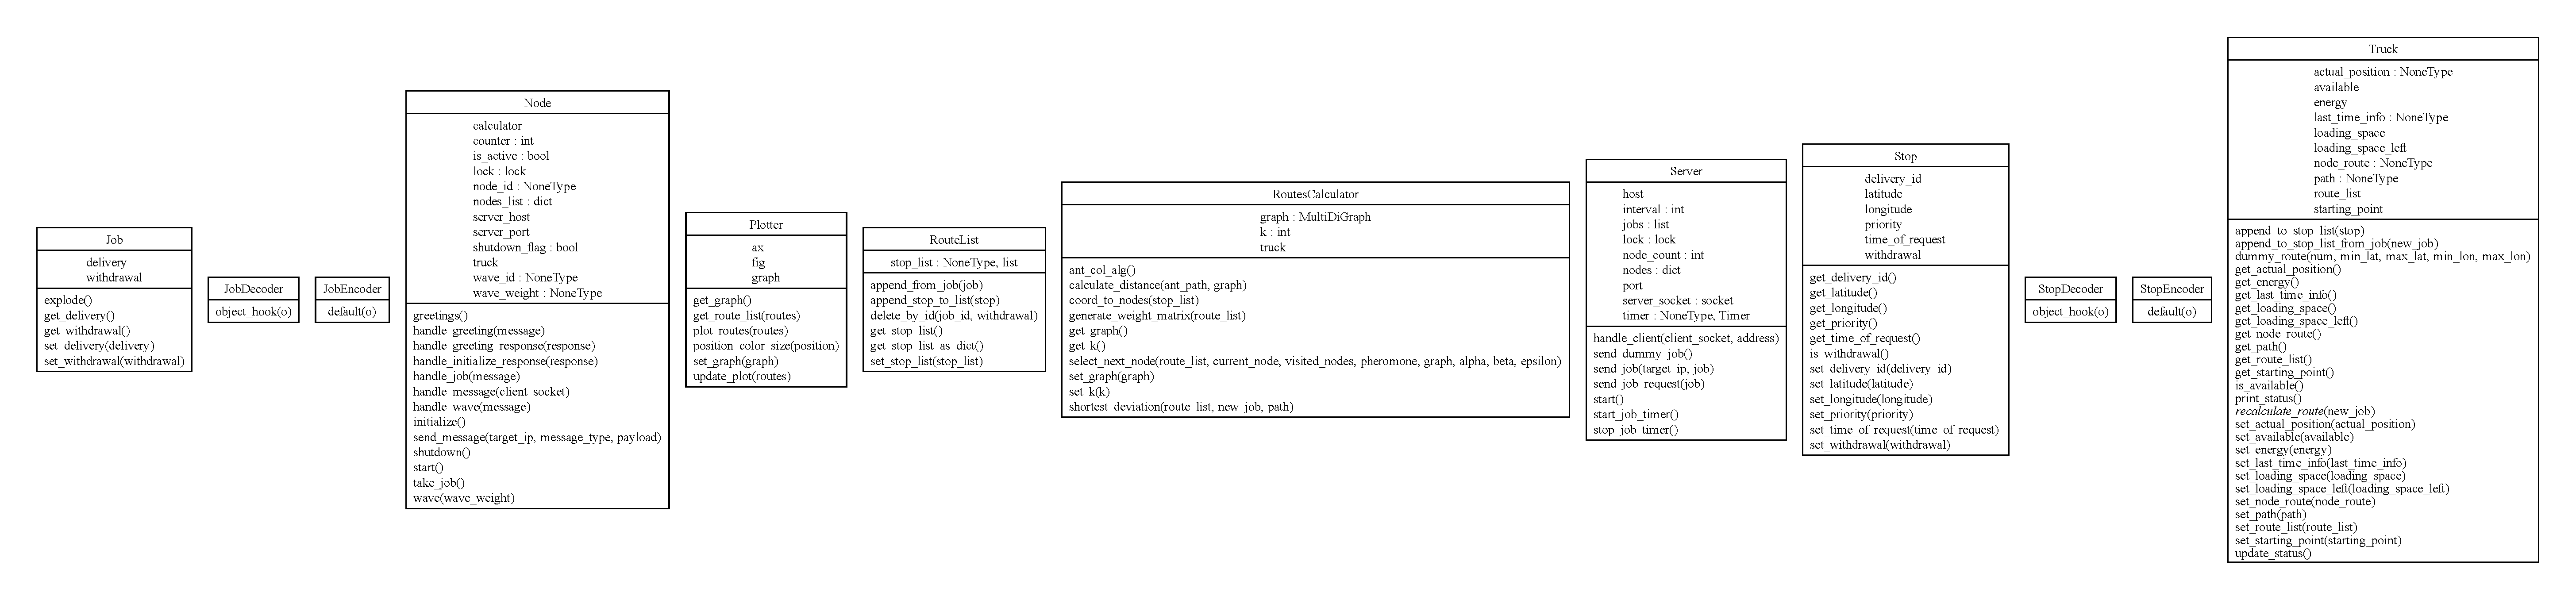
\includegraphics[trim={85cm 1cm 0 1cm}, clip, scale=.5]{img/classes.pdf}
    \caption{Attributes and methods of the Truck class}
    \label{fig:truck_class}
\end{figure}

\begin{itemize}
    \item \textbf{actual\_position}: A tuple containing the coordinates of the actual position of the vehicle.
    \item \textbf{available}: A boolean value that informs us of the status of the vehicle (True = available, False = not available).
    \item \textbf{energy}: The percentage of energy left to the vehicle. This might be useful in order to establish if the vehicle may take new orders or not.
    \item \textbf{last\_time\_info}: A timestamp needed to save the last time the vehicle updated its stats (mainly useful for debugging).
    \item \textbf{loading\_space}: The total loading space available to the vehicle.
    \item \textbf{loading\_space\_left}: The remaining loading space available to the vehicle.
    \item \textbf{node\_route}: This list of lists contains the information regarding the sorted path of the vehicle in a format readable by the OSMnx library.
    \item \textbf{path}: The sorted path of the vehicle.
    \item \textbf{route\_list}: The RouteList object of the vehicle.
    \item \textbf{starting\_point}: The coordinates of the starting point of the vehicle path. This would correspond to the warehouse or the depot where the vehicles are kept when not in use.
\end{itemize}

Aside from the setters and getters methods of the class we also implemented other methods useful for an abstract management of our resources, without need to access directly to the other classes.

\begin{itemize}
    \item \textbf{append\_to\_stop\_list}: This method directly calls the RouteList method append\_stop\_to\_list, to add to the vehicle route\_list object the new stop.
    \item \textbf{append\_to\_stop\_list\_from\_job}: This method directly calls the RouteList method append\_from\_job, to add to the vehicle route\_list object two new stops from a Job object.
    \item \textbf{dummy\_route}: This is a method useful for debugging. It returns us a specified number of fake Jobs, created from random coordinates in the format (latitude, longitude) in the interval [min\_lat, max\_lat] and [min\_lon, max\_lon].
    \item \textbf{print\_status}: In case we may need to print the stas of the vehicle in a human readable way (if the truck is running correctly, the actual timestamp, the energy left, the loading space left and the actual position of the vehicle).
    \item \textbf{recalculate\_route}: This is actually an unused method, but the idea would be to be able to call the methods needed to recalculate the route of the vehicle directly from the Truck object instead of calling them explicitly from RoutesCalculator.
    \item \textbf{update\_status}: This method currently just works for debugging: it reads the stats of the vehicle from a file, but ideally it would be a method that would work in a while loop reading the data from sensors on the vehicle.
\end{itemize}

\subsection{RoutesCalculator}
\begin{figure}[H]
    \centering
    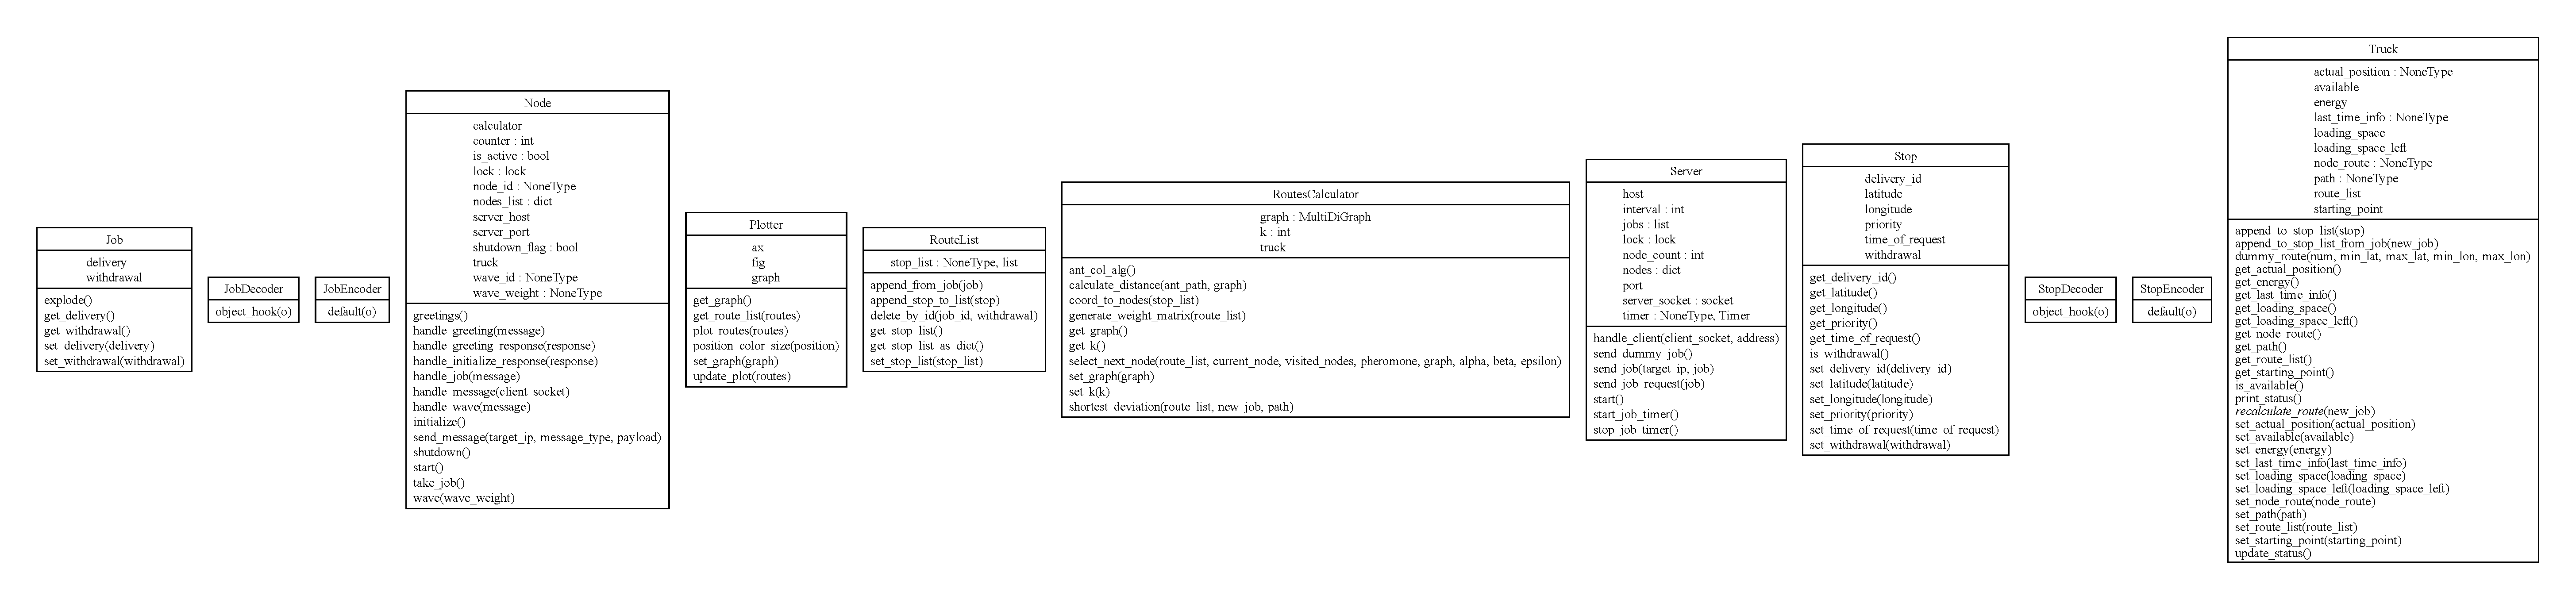
\includegraphics[trim={40.1cm 6.9cm 38cm 6.9cm}, clip, scale=.5]{img/classes.pdf}
    \caption{Attributes and methods of the RoutesCalculator class}
    \label{fig:routescalculator_class}
\end{figure}

\begin{itemize}
    \item \textbf{graph}: This is the OSMnx graph object, that is actually a NetworkX directed graph object. We obtain it from the OSMnx library passing directly the name of the place which we need the map of, specifyingwhat kind o graph we want, and then we call different methods to add to nodes and edges the values we need, like the edge weight based on the geographical distance between nodes.
    \item \textbf{k}: This value is currently unused, but it would be used in an hypothetical version of the RoutesCalculator object that allow us to calculate the best path considering the k shortest paths between each node. The reason why we did not implement it is because we need to keep performance in mind, and the ant colony algorithm in this implementation is already per se an algorithm with exponential computational complexity, and adding this variable to the algorithm would increase the exponential growth of the algorithm's complexity.
    \item \textbf{truck}: The Truck opject to which the calculator refers to. Thanks to this reference to the Truck object, the RoutesCalculator may read the attributes of the vehicle needed to compute the paths efficiently. We preferred to keep two separate objects as a modularity oriented design choice.
\end{itemize}

The following methods of this class are two main algorithms of the project, the ant colony algorithm and the greedy algorithm (shortest\_deviation), along with the other methods used to allow their use.

\begin{itemize}
    \item \textbf{ant\_col\_alg}: This is the main core of the project. It does not return a value, but directly sets the path and the node\_route attributes of the Truck object it refers to. This algorithm will be best explained in a further section.
    \item \textbf{calculate\_distance}: Subordinate method of ant\_col\_alg, it will also be best explained in a further section.
    \item \textbf{coord\_to\_nodes}: This method allow us to convert the human readable coordinates of the stops objects to node values, readable by the OSMnx library and the OSMnx graph object. It uses the nearest\_nodes OSMnx method.
    \item \textbf{generate\_weight\_matrix}: This method returns the weight matrix of the subgraph whose nodes are only our stop objects. It is basically an adjacency matrix where all the edges are characterized by the weight of the edge. Actually the specified weight measure for this is the distance between nodes, but the OSMnx method shortest\_path can take any weight as the cost measure for this optimization problem. The shortest\_path method uses the Dijkstra algorithm to find the optimal path between nodes; obviously this method's computational cost increases with the graph's dimension.
    \item \textbf{select\_next\_node}: Subordinate method of ant\_col\_alg, it will also be best explained in a further section.
    \item \textbf{shortest\_dev}: This method is a greedy algorithm that, having an already existing path and its cost, it adds a new withdrawal point in the path, just inserting it in the path, following the node closest to it. Then it does the same with the delivery point, searching the nearest node to it whose position in the path is set after the relative withdrawal. Then it computes the new weight of the path and returns it along the updated path (this method does not directly update the Truck object attributes because ideally it would first need to be elected by the network as the less costly path).
\end{itemize}

\subsection{Plotter}
\begin{figure}[H]
    \centering
    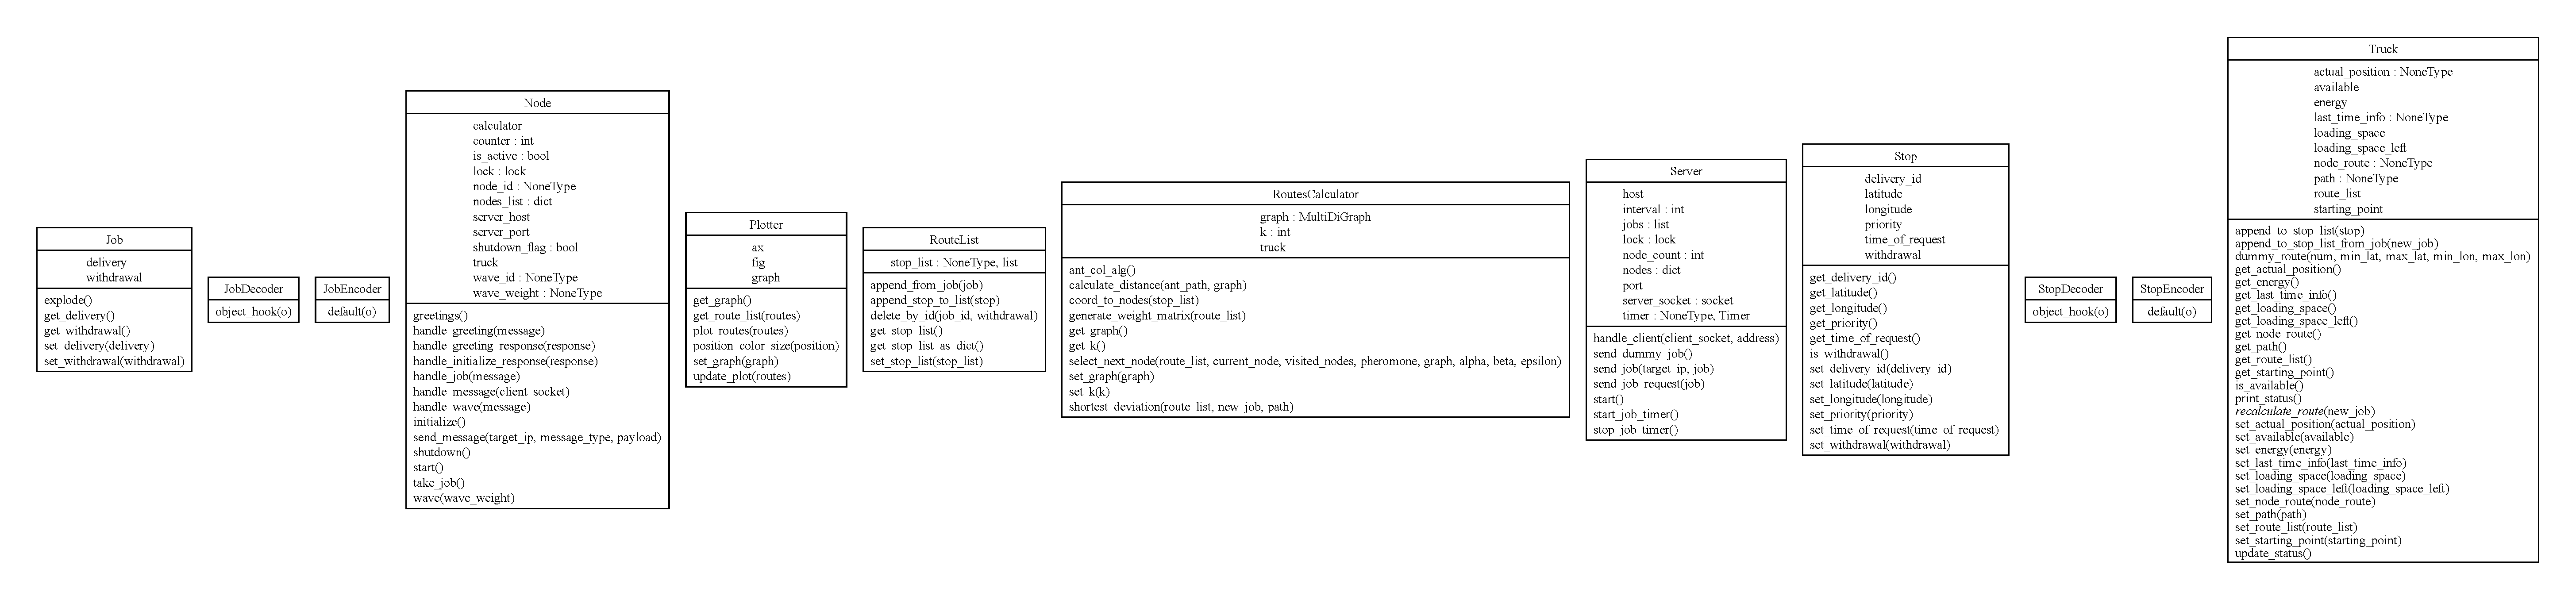
\includegraphics[trim={26cm 8cm 66cm 8cm}, clip, scale=.5]{img/classes.pdf}
    \caption{Attributes and methods of the Plotter class}
    \label{fig:plotter_class}
\end{figure}

This class is an helper for the plotting of the graph and the routes, it has no actual utility beside being a graphical tool for the project.

\begin{itemize}
    \item \textbf{ax, fig}: This are items used by the matplolib library to plot and update existing plots without having to delete them and then plot again.
    \item \textbf{graph}: This is the same OSMnx graph object used by RoutesCalculator.
\end{itemize}

\subsection{Node}
\begin{figure}[H]
    \centering
    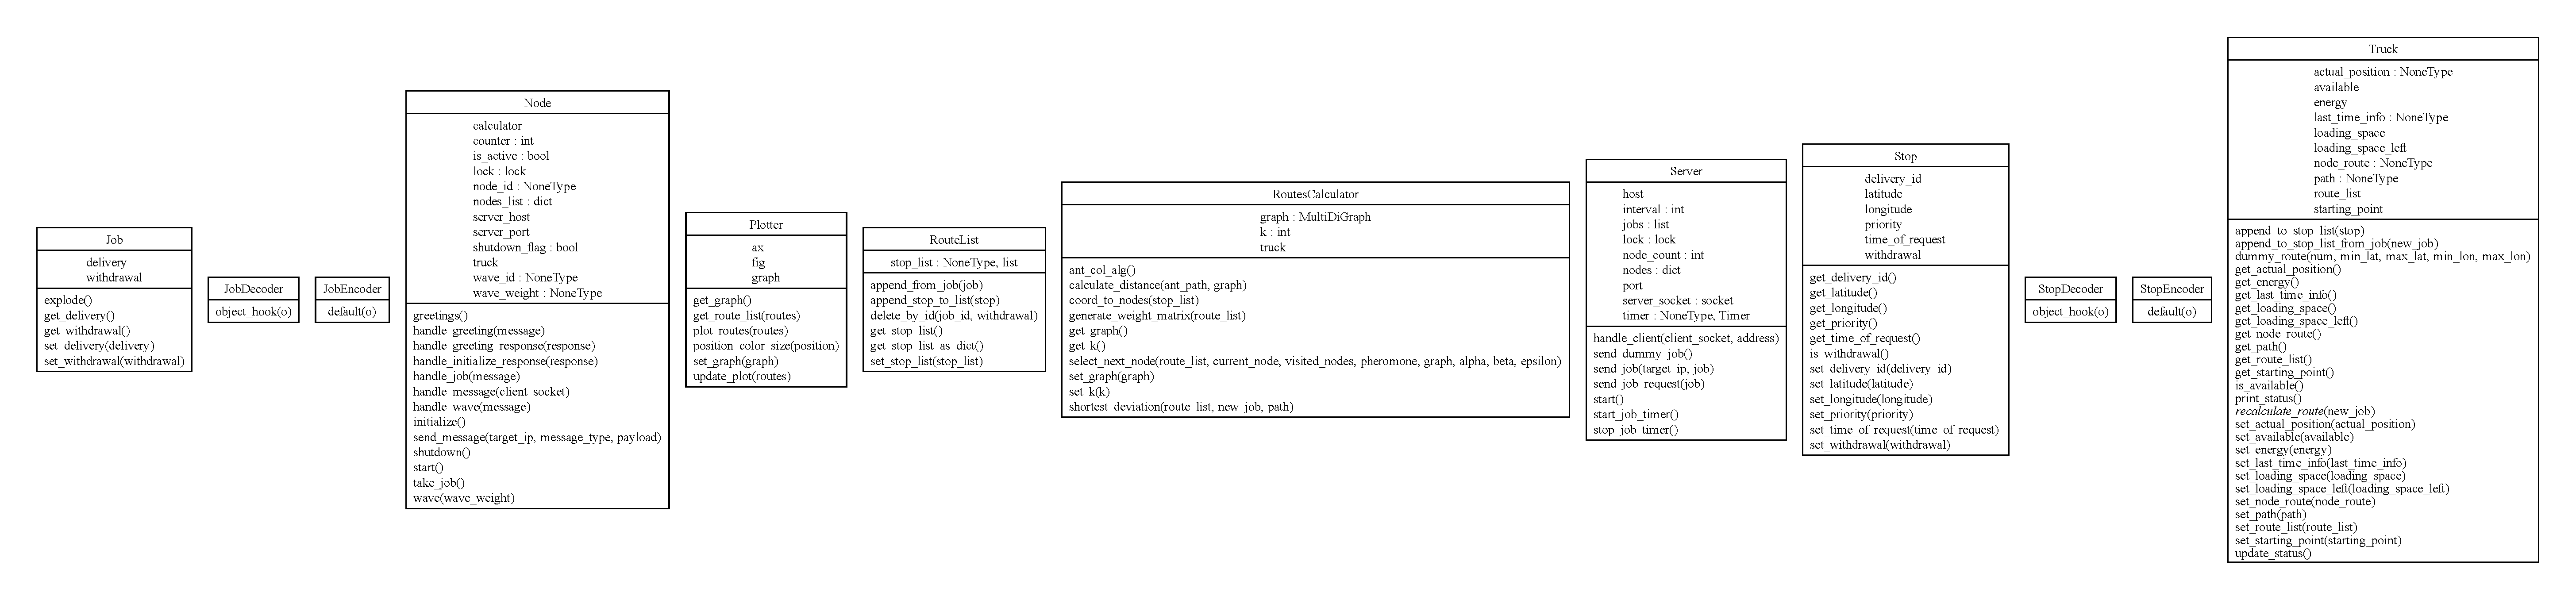
\includegraphics[trim={15cm 3cm 72.5cm 3cm}, clip, scale=.5]{img/classes.pdf}
    \caption{Attributes and methods of the Node class}
    \label{fig:node_class}
\end{figure}

This is the networking interface object for the vehicle used to communicate with the server and the other nodes; developed just for debugging purposes, it uses socket objects for communication.

\begin{itemize}
    \item \textbf{calculator}: This is a reference to the RoutesCalculator object used in the main program.
    \item \textbf{counter}: This is a counter for the wave algorithm implemented for the election of the node that will take a job request submitted by the server. When the counter reaches a value equal to the number of nodes in the network, it knows that it has been elected.
    \item \textbf{is\_active}: Flag value used to determine if the node is actually considerable active or not. Ideally this would be linked to certain vehicle's attributes like energy or storage left.
    \item \textbf{lock}: This object is used to allow threading in a safe way, avoiding race conditions to certain memory areas.
    \item \textbf{node\_id}: THe id of the node, given by the server, after joining the network.
    \item \textbf{nodes\_list}: The list of all the other nodes in the network, containing also information about the other nodes status.
    \item \textbf{server\_host}: The host of the server.
    \item \textbf{server\_port}: The port of the server.
    \item \textbf{shutdown\_flag}: This flag is used to gracefully shutdown the node functions and running threads. The threads while in their running loop always check if this flag is set to True, if so, they will stop working.
    \item \textbf{truck}: The reference to the Truck object.
    \item \textbf{wave\_id}: This is the id adopted by the node in the wave algorithm. When the algorithm starts, the wave\_id is equal to the node\_id, but if it adopts a new node election, then it will change its id to that node id.
    \item \textbf{wave\_weight}: This is the weight adopted by the node in the wave algorithm. When the algorithm starts, the wave\_weight is equal to the one computed by the node with the RoutesCalculator's shortest\_deviation method, but if it receives a message with a weight lower than its own, it will adopt that node election, changing its own wave\_weight to the that of that node.
\end{itemize}

The Node methods can be divided in two categories: the initialization methods and the wave methods.

The first category consists of communications between nodes and server to get initialized and the greetings messages to the other nodes.

The second category includes all the methods regarding the handling of a job request from the server and the subsequent wave algorithm with the other nodes.

\begin{itemize}
    \item \textbf{greetings}: The node, in this method, sends a greeting message to all the nodes it has in its node\_list. If after a timeout it does not receive an answer, it will mark the node as inactive.
    \item \textbf{handle\_greeting}: Upon receiving a greeting message, the node save the new node information in its node\_list and marks it as active. After that it responds with a greeting\_response message.
    \item \textbf{handle\_greeting\_response}: Upon receiving a greeting response, the node will mark the corresponding sender id in node\_list as active.
    \item \textbf{handle\_initialize\_response}: Upon receiving an initialize response, the node will save the received node list and its own new id.
    \item \textbf{handle\_job}: Upon receiving a job request from the server, the node will call the shortest\_deviation method from the RoutesCalculator object. After calculating the new weight, it will enter the wave algorithm.
    \item \textbf{handle\_message}: This is the method that gets called whenever the node receives a message. Depending on the type of message it will call a different handler.
    \item \textbf{handle\_wave}: Upon receiving a wave message, one of the following cases will occur:
    \begin{itemize}
        \item The received wave\_id is equal to the node id: discard the message and increment the counter.
        \item The received wave\_id is equal to the node wave\_id: discard the message.
        \item The received wave\_weight is grater than the node wave\_weight: discard the message.
        \item The received wave\_weight is lower than the node wave\_weight: adopt the received wave\_id and wave\_weight, then broadcast a wave message with the new wave information.
    \end{itemize}
    When the counter of one node will reach the number of nodes in the network minus one, this means that it has been elected and it will now call the take\_job method. It is safe that it will never happen that more than one node will be elected in the same wave algorithm.
    \item \textbf{initialize}: This method sends to the server an initialize message that starts our three-way handshake. After sending it, it waits for the response from the server, and once it receives it, it will call the handle\_initialize\_response.
    \item \textbf{send\_message}: This is the method used by the node when it needs to send a message. We simply pass the target address, the type of message and the payload.
    \item \textbf{shutdown}: This method simply sets the shutdown flag to True, initializing the shutdown sequence of the node.
    \item \textbf{start}: This method is called when the node is initialized. It will start the initialize thread and the greetings thread after that. It also binds the socket and starts listening for messages.
    \item \textbf{take\_job}: This method gets called when a node gets elected in the wave algorithm. It will send a take job message to the server.
    \item \textbf{wave}: The wave algorithm starts initializing the counter at $0$, initializing the wave\_id with the node\_id, and initializing the wave\_weight with the result of shortest\_deviation passing the new Job object. After that it sends a message with its wave\_id and wave\_weight to all other nodes.
\end{itemize}

\subsection{Server}
\begin{figure}[H]
    \centering
    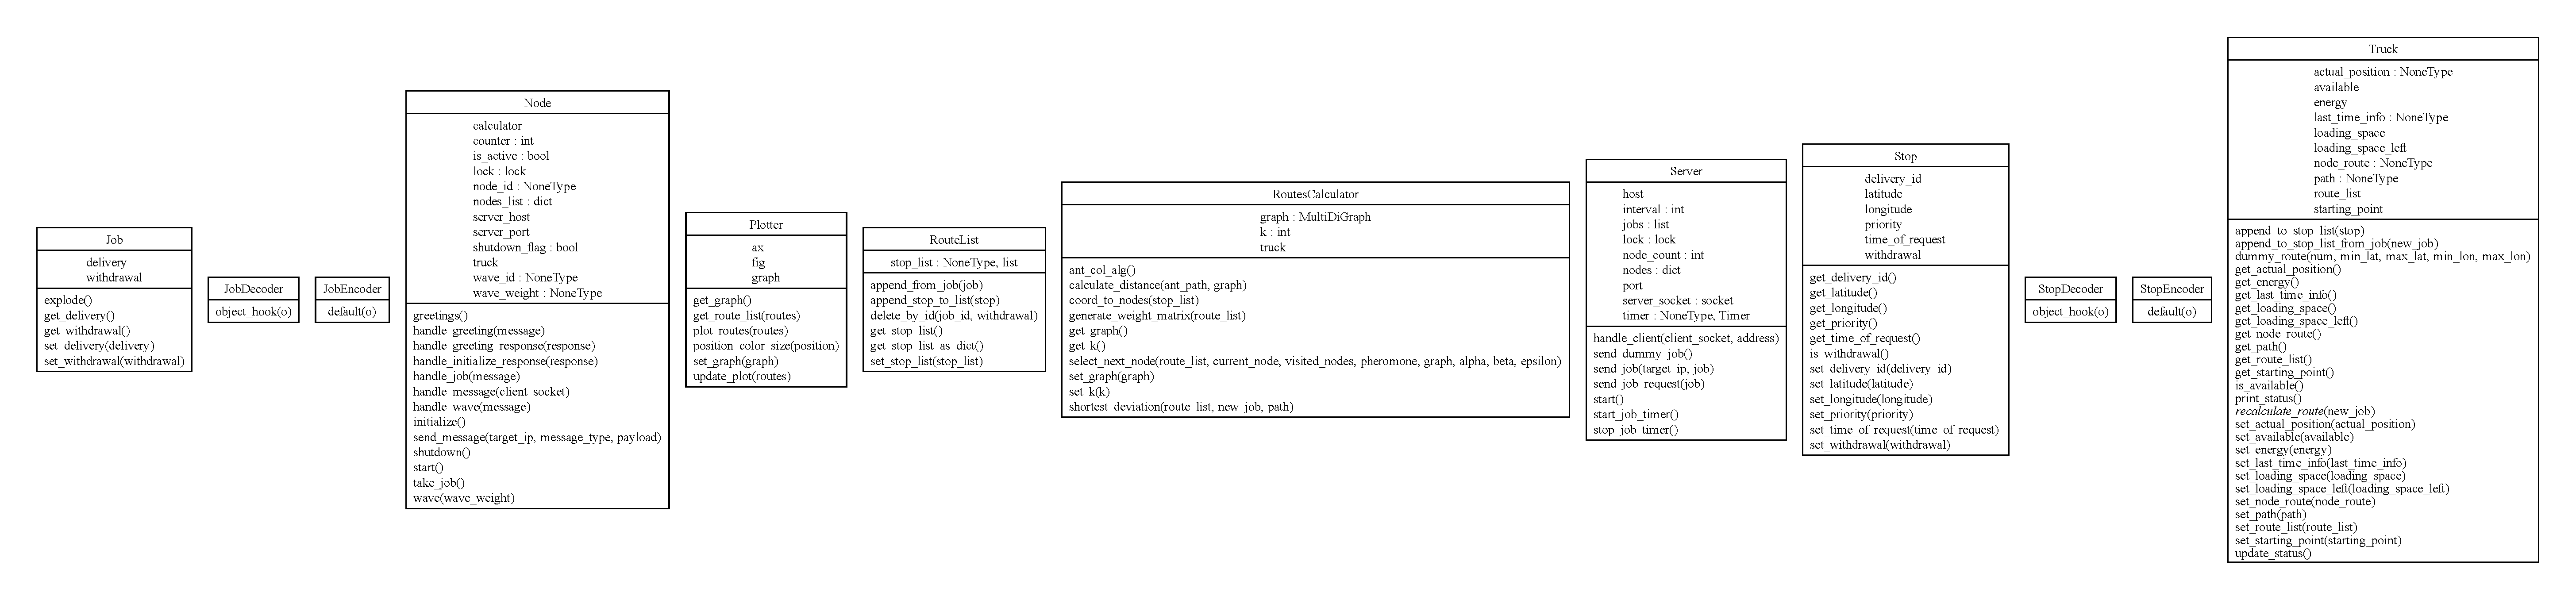
\includegraphics[trim={60.4cm 6cm 30cm 6cm}, clip, scale=.5]{img/classes.pdf}
    \caption{Attributes and methods of the Server class}
    \label{fig:server_class}
\end{figure}

The server implementation is pretty simple, we just used it for debugging purposes.

\begin{itemize}
    \item \textbf{host}: The server host.
    \item \textbf{interval}: The timeout limit.
    \item \textbf{jobs}: The server uses this attribute to keep track of the jobs currently being executed by the nodes.
    \item \textbf{lock}: This object is used to allow threading in a safe way, avoiding race conditions to certain memory areas.
    \item \textbf{node\_count}: The number of nodes in the network.
    \item \textbf{nodes}: The dictionary containing the nodes\_id and their relative ips.
    \item \textbf{port}: The server port.
    \item \textbf{server\_socket}: The socket that gets initialized in the constructor with the passed host and port.
    \item \textbf{timer}: The timer object needed for the timeout waiting a response.
\end{itemize}

The server implements the following methods that mainly regards the handling of the node initialization and the handling of the job requests.

\begin{itemize}
    \item \textbf{handle\_client}: This method handle the messages from the client:
    \begin{itemize}
        \item If the message is an initialization message, the server checks if the ip of the node is already in its nodes list, if not it increases the node\_count, adds the node ip and id to its list, and then it sends a response containing the assigned id and the nodes list. If the node is already in the nodes list, the server will respond with an error.
        \item If the message is a take\_job request, it will respond with an ack.
    \end{itemize}
    \item \textbf{send\_dummy\_job}: This method is for debugging purposes only. It creates a fake Job object with random coordinates and calls the send\_job method.
    \item \textbf{send\_job}: The server sends the Job object in a job type message in broadcast to the network.
    \item \textbf{send\_job\_request}: The server calls the send\_job method in a for loop for every node in the nodes list.
    \item \textbf{start}: The initialization method for the server, that puts it listening for messages from the clients.
    \item \textbf{start\_job\_timer}: The method to start the timer.
    \item \textbf{stop\_job\_timer}: The method to stop the timer.
\end{itemize}

\subsection{Github}
The project files can be found at this GitHub \href{https://github.com/MTheHead61/DS_project.git}{link}.

\section{Centralized vs decentralized approach}
Aside from our implementation, we should make a few considerations about the differences between the centralized and decentralized approach.

What we implemented is sorta of an hybrid approach, with a first computation of the vehicle paths, using the ant colony algorithm on the server, and then the computation of a possible deviation on the vehicle themselves. Aside from the academic point of view, in a real life scenario we should investigate the advantages and downsides of a pure centralized approach and a pure decentralized approach.

The two main criteria that might come to mind are fault tolerance and real time computations.

Of course having a fully distributed and decentralized system would mean having no central server and that the network created by the vehicles would be the full network: we would have to implement a mechanism to elect a node as leader in our network. In this case probably we would use a consensus algorithm like raft, and then we would let every node make the pathfinding computations locally, and then inform the leader, that would register the events and then inform the nodes of the new log. The advantages are pretty clear: we would have a system that would be extremely resilient to faults: if a node would fail, the leader node would discover it and inform the others, letting them take the jobs of the other node, computing new routes. If it would be the leader node to fail, it would just take another round of election and we would have a new leader node, and then do the same, splitting the jobs with the other nodes. The real problem would be related to the computational weight of the pathfinding operations: on a server machine these would take seconds at most (without considering that if we would have also to query the geocoder and recompute the weight matrix the problem would scale exponentially), but on a smaller device it would probably take a lot than that, making us consider a new plethora of problems like computing with respect to the future position of the vehicle, estimating the computation times, wasting computation resources on a mobile machine, wasting also energy that could be used for something else.

Instead, in a fully centralized approach we would have a central server doing all the pathfinding computations. When a new job request would arrive it would compute all the deviations for every active vehicle and then notify the chosen vehicle of the new stop. The vehicle could will be able to refuse (low battery or no storing space), and then the server would still be able to notify the next lowest weight deviation vehicle. The greatest advantage of this approach is obvious: the heavy computations would run exclusively on a powerful server machine, probably taking still less time than parallelizing the $N$ computations on $N$ extremely less powerful machines. The compromise would be losing all of the fault tolerance from the decentralized approach, having one critical fault point on the server. This of course can be bypassed with various strategies (back-up machines for example), making the overall system more resilient.

In general probably the best approach in a real life implementation would still be the fully centralized one: we would have to lose a bit of fault tolerance in order to have a more robust (computationally-wise) system, that would also severely simplify the networking approach, eliminating all the need for the nodes to communicate between themselves.

\section{The ant colony algorithm}
The main purpose of this project is to test the performance of the \textbf{ant colony algorithm} in the already presented scenario of a fleet of vehicles that must divide their load of work in a functional way. This means that we want that the algorithm is able to minimize the weight we are considering for this optimization problem, and that eventually the split weight can have a variance as low as possible.

As we already explained, the ant colony algorithm draws inspiration from the foraging behavior of ants. In nature, ants communicate through pheromones, leaving a trail as they find food. This trail attracts other ants, reinforcing the path to the food source. The algorithm translates this concept into an optimization algorithm where artificial ants navigate a solution space, leaving digital "pheromones" on the paths they explore.

So basically we are deploying artificial ants searching for the optimal solution to a problem. Initially, the artificial ants are scattered randomly across the solution space. Pheromone levels are initialized uniformly on all paths. Each ant then starts to construct a solution by iteratively choosing the next component based on a combination of pheromone levels and heuristic information.

The pheromone levels represent the desirability of a particular path, analogous to the attractiveness of a trail in the natural world. Heuristic information guides the ants toward promising regions in the solution space, akin to ants being drawn to areas where they are likely to find food.

As the ants construct solutions, they deposit pheromones on the paths they traverse. The better the solution, the more intense the pheromone deposition. This imitates the reinforcement of successful paths in nature. Over time, paths leading to superior solutions accumulate more pheromones, making them more appealing to subsequent ants.

To prevent the algorithm from converging prematurely, pheromones are subjected to evaporation. This simulates the natural decay of pheromone trails and ensures adaptability in the exploration process. The balance between exploration and exploitation is crucial in the ant colony algorithm. Initially, there's a phase of exploration where ants discover diverse paths. As the algorithm progresses, the influence of pheromones causes a shift towards exploitation, where ants favor paths with higher pheromone levels.

The convergence to a solution is a dynamic interplay between the ants' exploration and exploitation tendencies. The collective intelligence emerges as ants communicate indirectly through the pheromone-laden paths. Paths that consistently lead to better solutions intensify in attractiveness, guiding subsequent ants to explore similar routes.

The implementation that we will show in this section is not the same of the previous section, but a modified version used for the case study presented in the following section.

\subsection{Prelude}
\begin{python}
import osmnx as ox
import numpy as np
import geocoder
import pandas as pd
import copy
import datetime
import matplotlib.pyplot as plt

import itertools
\end{python}

These are all the libraries we are importing for the experiment:
\begin{itemize}
    \item \textbf{osmnx}: as we said before this is a library that uses Open Street Map data and manages it using the NetworkX library.
    \item \textbf{numpy}: python library that allows to manage scientific data and scientific computing with ease.
    \item \textbf{geocoder}: geocoding library for python, it allows us to get coordinates from addresses.
    \item \textbf{pandas}: python library used to manage dataframes.
    \item \textbf{copy}: this python library is extremely useful with its deepcopy function to set a variable to a specific value of another object without passing the reference of said object.
    \item \textbf{datetime}: the standard python library to get times and manage time variables.
    \item \textbf{matplotlib}: python library for plotting data and manage plots.
    \item \textbf{itertools}: this library has many functions used to create iterable items, we use it mainly for the cartesian product of the ant colony algorithm's parameters for the grid search of the optimal parameters.
\end{itemize}

\begin{python}
jobs_dataframe = pd.read_excel('complete_original_task_list.xlsx')
\end{python}

We use pandas function to pass the excel data to a dataframe, so we can read it and feed it to the algorithm after some management. We also had to correct some typos making researches on the web, since some of these addresses did not gave us a result on the geocoding queries, but we will see it in detail in the study case section.

\begin{python}
G = ox.graph_from_point((45.464664, 9.188540), dist=20000, network_type='drive', simplify=False)

G = ox.distance.add_edge_lengths(G)
G = ox.speed.add_edge_speeds(G)
G = ox.speed.add_edge_travel_times(G)
\end{python}

These lines of code will give us the graph with all the information we need for our ant colony algorithm:
\begin{itemize}
    \item \textbf{graph\_from\_point} is a function that returns us a graph starting from a certain set of coordinates for a certain km range. We also specify the type of network we are interested in (if we want just drive roads, pedestrian roads, both etc) and if we want to simplify the edges removing some of the less important ones.
    \item \textbf{add\_edge\_lengths}: adds the length of the road stat to the edges.
    \item \textbf{add\_edge\_speeds}: adds the speed limit stat to the edges.
    \item \textbf{add\_edge\_travel\_times}: adds the mean time travel stat to the edges.
\end{itemize}

\subsection{Ant Colony Algorithm}
We will now proceed to show all the code related to the ant colony algorithm.

\begin{python}
def get_jobs(df = jobs_dataframe, graph = G, starting_point = 272714832):
    job_list = []
    ref_map = {'Via Olona, 2, 20123 Milano MI, Italy': {'id': 0, 'has_pick_up': True}}
    map_value = 1

    job_list.append({'id': 0, 'pick_up': True, 'node': starting_point})
    
    for i, row in df.iterrows():
        job = {}
        if row['Reference'] not in ref_map:
            ref_map[row['Reference']] = {}
            ref_map[row['Reference']]['id'] = map_value
            ref_map[row['Reference']]['has_pick_up'] = False
            map_value += 1
        job['id'] = ref_map[row['Reference']]['id']
        if row['Category']=='drop_off':
            job['pick_up'] = False
        else:
            job['pick_up'] = True
            ref_map[row['Reference']]['has_pick_up'] = True
        g = geocoder.osm(row['Address']).json
        job['node'] = ox.distance.nearest_nodes(graph, g['lng'], g['lat'])
        job_list.append(job)

    for k in ref_map:
        if ref_map[k]['has_pick_up']:
            continue
        else:
            job_list.append({'id': ref_map[k]['id'], 'pick_up': True, 'node': 272714832})

    return job_list, ref_map
\end{python}

This first function returns us a list of dictionary items starting from the dataframe we obtained earlier. Basically the way it works is, fixed a starting point, that will be the node $0$ of our matrix, the function maps the dataframe reference values and translates them in int values, then queries the geocoder to obtain the coordinates of the address, and uses those coordinates to get the corresponding nodes on the graph. In the end, it checks if there are no "orphan" delivery orders, and in that case we will assume that the shipment relative to that delivery has been picked up before and is waiting for delivery in the warehouse, so we will add a dummy job placed in the starting point/warehouse to fill in the gap of the missing pick up.

\begin{python}
def get_weight_matrix(G, job_list, weight_string='travel_time'):
    l = len(job_list) #The number of jobs
    paths_dict = {}
    weight_matrix = np.zeros((l, l)) #Initialize the matrix
    for i in range(l): #For every job (rows)
        paths_dict[i] = {}
        for j in range(l): #For every job (columns)
            if i != j: #row not equal column, no self loops in the adjacency matrix
                el = ox.routing.shortest_path(G, job_list[i]['node'], job_list[j]['node'], weight=weight_string, cpus=None) #Open Street Map uses Dijkstra's algorithm in order to find the path between two nodes that minimize the chosen weight
                paths_dict[i][j] = el
                for u, v in zip(el, el[1:]): #Use the zip function to create an iterable object for every step of the path
                    weight_matrix[i][j] += G.edges[u,v,0][weight_string] #For every step of the path add the weight to the matrix
    return weight_matrix, paths_dict #Return the weight matrix
\end{python}

This is without a dubt the most computastional heavy function of the whole project, but it is necessary to obtain the weights of the travel between nodes. It is of course heavy because we will have to run the Dijkstra's algorithm (as we can read in the comments of the code) $N^2$ times, for $N$ equal to the number of nodes, for a non-negligible amount of edges. Luckily we can parallelize it (cpus=None).

From this point on all the functions we will see are used directly in the ant colony algorithm, describing each fundamental part of it. Since all the functions are heavily commented, we will be very brief on the comments.

\begin{python}
def get_allowed_nodes(job_list, path, visited_nodes):
    allowed_nodes = [] #Initialize the allowed nodes list
    for i in range(len(job_list)): #For every possible job
        if i in visited_nodes: #If it has already been visited
            continue #Skip iteration
        if job_list[i]['pick_up']: #If it is a pick up
            allowed_nodes.append(i) #Append the node to the allowed nodes
        else: #Otherwise, if it is not a pick up
            for node in path: #For every node already visited
                if job_list[node]['id'] == job_list[i]['id']: #If the node already visited the relative withdrawal
                    allowed_nodes.append(i) #Append the node to the allowed nodes
    return allowed_nodes #Return the allowed nodes list
\end{python}

This function simply returns a list of all the nodes that an ant, given its path up to that point and given the other's concurrent ants path, can travel to.

\begin{python}
def get_next_node(weight_matrix, job_list, pheromone, path, visited_nodes, epsilon, alpha, beta):
    current_node = path[-1] #The node we are currently in is the last visited
    allowed_nodes = get_allowed_nodes(job_list, path, visited_nodes) #Get the list of allowed nodes
    if len(allowed_nodes) == 0: #If the allowed nodes list is empty
        return False #Return false
    pheromone_values = pheromone[current_node, allowed_nodes] #Extract the pheromone values of the outgoing edges of this node
    heuristic_values = 1 / (weight_matrix[current_node, allowed_nodes] + epsilon) #Compute the heuristic values as the inverse of the weights
    #heuristic_values *= priorities #If there were some priorities to slide in the equation, they would need to be computed here
    probability_values = (pheromone_values ** alpha) * (heuristic_values ** beta) #Initialize the probability values as the pheromones at power alpha times heuristic values at power beta
    probability_values /= np.sum(probability_values) #Normalize the probability values
    next_node = np.random.choice(allowed_nodes, p=probability_values) #Based on probability values choose the next node
    return next_node #Return the next node
\end{python}

This function, given the allowed nodes an ant can travel to, does a random choice of the next node in its path. The choice, although being random, it has a weighted probability, given by the following formula:
\begin{equation}
    p_n = {pher}^{\alpha}h^{\beta}
\end{equation}
where $p_n$ is the non-normalized probability, ${pher}$ is the pheromone value, $h$ is the inverse of the weight and $\alpha$ and $\beta$ are their respective exponents.

\begin{python}
def compute_path_weight(weight_matrix, ant_path):
    tot_weight = 0 #Initialize weight
    n_weights = {}
    for n in ant_path: #For every agent's path
        weight = 0
        for i in range(len(ant_path[n]) - 1): #For every edge in agent's path
            weight += weight_matrix[ant_path[n][i], ant_path[n][i + 1]] #Add the edge weight
        n_weights[n] = weight
        tot_weight += weight
    return tot_weight, n_weights #Return the total sum of paths' weight
\end{python}

After all the concurrent ants terminate their travel we need to compute their path weight. We made sure to have the algorithm returns both the total weight of the concurrent ants and their individual scores.

\begin{python}
def update_pheromone(pheromone, ant_paths, ant_weights, ant_n_weights, rho, use_sum_weight=True):
    new_pheromone = pheromone #Initialize new pheromone levels
    new_pheromone *= (1 - rho) #Apply decay rate
    for i in range(len(ant_paths)): #For each ant
        for n in ant_paths[i]: #For each agent in ant_path
            for u, v in zip(ant_paths[i][n], ant_paths[i][n][1:]): #Use zip in order to create an iterable of the path
                if use_sum_weight:
                    new_pheromone[u, v] += 1 / ant_weights[i] #Add pheromone values for each edge traveled inverse to the total weight of the path traveled
                else:
                    new_pheromone[u, v] += 1 / ant_n_weights[i][n] #If we would prefer to update the pheromones using the individual weights we would need to do it this way
    return new_pheromone
\end{python}

The update pheromone function is pretty straightforward too. We apply the decay we defined ($1-\rho$), then we just add new values to the existing ones based on the inverse of the weights of the road traveled. We implemented two different methods to update the pheromones, based on the idea that updating the pheromone with the sum of the weights of the concurrent ants might give us a different result then updating them with the singular weights of every ant. We expect the algorithm to converge more efficiently towards a global minimum if we update the pheromones with the singular weight values of each ant.

\begin{python}
def ant_colony(G, job_list, weight_matrix, n_agents=4, n_ants=10, n_iterations=50, alpha=1, beta=2, rho=0.5, pher_sum_weight=True):
    '''
    G = the osm graph
    n = number of agents for the algorithm
    n_ants = number of ants running for iteration
    n_iteration = number of iterations to let the algorithm converge
    alpha = exponent of the pheromone (higher values give pheromone more weight)
    beta = exponent of the cost measure (higher values give more weight to the cost)
    rho = pheromone decay rate ([0,1] where 0 lefts the pheromone values unchanged)
    '''
    epsilon = 1e-10 #This value is added to the denominator in the divisions to avoid divisions by zero
    #weight_matrix = get_weight_matrix(G, job_list) #The weight matrix obtained from the function
    #Since the computation for the weight matrix is very heavy we prefer, for debugging purposes, to compute it outside the main algorithm use the one passed as parameter
    pheromone = np.ones_like(weight_matrix) * 0.1 #Initialize the pheromones matrix
    # Define the main algorithm loop
    results = {"path": [], "weight": [], "n_weights": []} #Initialize results dictionary
    for iteration in range(n_iterations): #For every iteration
        ant_paths = [] #Initialize the list of paths
        ant_weights = [] #Initialize the list of weights
        ant_n_weights = [] #Initialize the list of weights for every agent
        for ant in range(n_ants): #For every ant
            ant_path = {} #Initialize path
            for n in range(n_agents): #For every agent
                ant_path[n]=[0] #Start the path from the starting node
            n = -1 #Initialize the agents iterator
            visited_nodes = [0] #Initialize the visited nodes list
            end_path = [False] * n_agents #List to check if an agent has already ended its path
            while len(visited_nodes) < len(job_list): #Until all nodes are visited
                n = (n + 1) % n_agents #Changing agent at each iteration
                if end_path[n]: #If the ant has already ended its path
                    continue #Skip the loop iteration
                next_node = get_next_node(weight_matrix, job_list, pheromone, ant_path[n], visited_nodes, epsilon, alpha, beta) #Select the next node
                if next_node == False: #If the next_node function returns False
                    end_path[n] = True #Set the end_path for this agent to True
                    ant_path[n].append(0) #End the path going back to the starting point
                    continue #Skip the loop iteration
                ant_path[n].append(next_node) #Append the node to the path of the agent
                visited_nodes.append(next_node) #Update the list of visited nodes
            for e in range(len(end_path)): #For every agent
                if end_path[e] == False: #Check if the path ended at the warehouse
                    ant_path[e].append(0) #If not, append the end point of the path
            ant_paths.append(ant_path) #Save the path
            weight, n_weights = compute_path_weight(weight_matrix, ant_path)
            ant_weights.append(weight) #Save the weight of the path
            ant_n_weights.append(n_weights) #Save the individual weights of the agents
        pheromone = update_pheromone(pheromone, ant_paths, ant_weights, ant_n_weights, rho, use_sum_weight=pher_sum_weight) #Update pheromones on the edges of the graph
        best_ant_index = np.argmin(ant_weights) #Find the best ants
        best_ant_path = ant_paths[best_ant_index] #Find the best path
        best_ant_weight = ant_weights[best_ant_index] #Find the weight of the best ant
        best_ant_n_weights = ant_n_weights[best_ant_index] #Finde the individual weights of the best ant
        results["path"].append(best_ant_path) #Append best ant path to results
        results["weight"].append(best_ant_weight) #Append best ant weight to results
        results["n_weights"].append(best_ant_n_weights) #Append best individual weight to results
    return results
\end{python}

The main function of the algorithm basically just puts everything together: for every iteration, for every ant we travel through our subgraph until we traveled it all, than we compute our weights, update the pheromones and find the best ant of the iteration, saving its result. The result this function returns is a list of the best ant for each iteration. Normally from this we simply get the best solution based on our criteria.

\subsection{Experiment}
All of the following code will present also the instructions to calculate its computing time.

First of all, since, as we said, the computation of the weight matrix is very computationally heavy, we do it before the ant colony algorithm, instead of doing this at run time.
\begin{python}
start = datetime.datetime.now()

weight_matrix, shortest_paths = get_weight_matrix(G, job_list)

end = datetime.datetime.now()
weight_matrix_time = end-start
\end{python}

After that we can begin our grid search, searching for the optimal set of parameters for our problem:

\begin{python}
n_ants_list=[10, 20, 30, 40, 50]
n_iterations_list=[50, 100, 150, 200, 250]
alpha_list=[0.0, 0.2, 0.5, 1.0, 2.0, 5.0]
beta_list=[0.0, 0.2, 0.5, 1.0, 2.0, 5.0]
rho_list=[0.0, 0.001, 0.01, 0.1, 0.5, 0.9]
pher_sum_weight_list=[False, True]

grid_search = itertools.product(n_ants_list, n_iterations_list, alpha_list, beta_list, rho_list, pher_sum_weight_list)

grid_search_num = len(list(itertools.product(n_ants_list, n_iterations_list, alpha_list, beta_list, rho_list, pher_sum_weight_list)))

ant_colony_time = {}

results = {}

grid_iteration = 1

for params in grid_search:

    n_ants, n_iterations, alpha, beta, rho, pher_sum_weight = params

    print(f"{grid_iteration}/{grid_search_num}: n_ants = {n_ants}, n_iterations = {n_iterations}, alpha = {alpha}, beta = {beta}, rho = {rho}, pher_sum_weight = {pher_sum_weight}")
    
    start = datetime.datetime.now()
    
    res = ant_colony(G, job_list, weight_matrix, 4, n_ants, n_iterations, alpha, beta, rho, pher_sum_weight)
    
    end = datetime.datetime.now()
    
    ant_colony_time[params] = end-start
    results[params] = res

    grid_iteration +=1
\end{python}

Basically we initialize the algorithm parameters list, with all the values we want to try, then we compute a cartesian product of those parameters (itertools.product), and for every combination of those parameters we run the ant colony algorithm, searching for the set of parameters that will give us the optimal solution.

\section{Study case}
Our study case involves a dataset from a real business located in Milan, Italy.

\begin{table}[H]
\centering
\begin{adjustbox}{max width=\textwidth}
\begin{tabular}{rllrrllrlllr}
\toprule
Id & Reference & Address & Start travel & End travel & Start task & End task & Duration & Category & Start large & End large & Complete range \\
\midrule
0 & Frida's Corso Genova02\_2023-11-21 & Via Ettore Ponti, 58, Milano, MI, Italia & 0 & 0 & 2023-11-21 15:00:00 & 2023-11-21 17:00:00 & 0.003472 & drop\_off & 2023-11-21 15:00:00 & 2023-11-21 17:00:00 & 0.083333 \\
1 & Frida's Corso Genova02\_2023-11-21 & Corso Genova, 6, 20123 Milano MI, Italy & 0 & 0 & 2023-11-21 12:15:00 & 2023-11-21 15:00:00 & 0.003472 & pick\_up & 2023-11-21 12:15:00 & 2023-11-21 15:00:00 & 0.114583 \\
2 & Fiori Fumagalli03\_2023-11-21 & Foro Buonaparte, 22, Milano, MI, Italia & 0 & 0 & 2023-11-21 14:15:00 & 2023-11-21 17:00:00 & 0.003472 & drop\_off & 2023-11-21 14:15:00 & 2023-11-21 17:00:00 & 0.114583 \\
3 & Cafezal02\_2023-11-21 & Via Larga, 13, Milano, MI, Italia & 0 & 0 & 2023-11-21 12:15:00 & 2023-11-21 17:00:00 & 0.003472 & drop\_off & 2023-11-21 12:15:00 & 2023-11-21 17:00:00 & 0.197917 \\
4 & Clori03\_2023-11-21 & Via Larga, 19, Milan, Metropolitan City of Milan, Italy & 0 & 0 & 2023-11-21 12:00:00 & 2023-11-21 17:00:00 & 0.003472 & drop\_off & 2023-11-21 12:00:00 & 2023-11-21 17:00:00 & 0.208333 \\
5 & Fiori Fumagalli03\_2023-11-21 & Via Messina, 47, Milano, MI, Italia & 0 & 0 & 2023-11-21 17:30:00 & 2023-11-21 18:00:00 & 0.003472 & drop\_off & 2023-11-21 17:30:00 & 2023-11-21 18:00:00 & 0.020833 \\
6 & Fiori Fumagalli03\_2023-11-21 & Piazza Guglielmo Oberdan, 2, Milano, MI, Italia & 0 & 0 & 2023-11-21 14:00:00 & 2023-11-21 16:15:00 & 0.003472 & pick\_up & 2023-11-21 14:00:00 & 2023-11-21 16:15:00 & 0.093750 \\
7 & La teiera Eclettica01\_2023-11-21 & Via Piero della Francesca, 74, Milano, MI, Italia & 0 & 0 & 2023-11-21 14:00:00 & 2023-11-21 17:00:00 & 0.003472 & drop\_off & 2023-11-21 14:00:00 & 2023-11-21 17:00:00 & 0.125000 \\
8 & La teiera Eclettica01\_2023-11-21 & La Teiera Eclettica, Via Melzo, 30, Milano, MI, Italia & 0 & 0 & 2023-11-21 11:00:00 & 2023-11-21 16:00:00 & 0.003472 & pick\_up & 2023-11-21 11:00:00 & 2023-11-21 16:00:00 & 0.208333 \\
9 & Dolcemente01\_2023-11-20 & Via Mario Pichi, 8, Milano, MI, Italia & 0 & 0 & 2023-11-21 11:00:00 & 2023-11-21 17:00:00 & 0.003472 & drop\_off & 2023-11-21 11:00:00 & 2023-11-21 17:00:00 & 0.250000 \\
10 & Florarredo01\_2023-11-21 & Via Gaetano de Castillia, 6A, Milano, MI, Italia & 0 & 0 & 2023-11-21 11:00:00 & 2023-11-21 17:00:00 & 0.003472 & drop\_off & 2023-11-21 11:00:00 & 2023-11-21 17:00:00 & 0.250000 \\
11 & Florarredo01\_2023-11-21 & Piazza della Repubblica, 32, 20124 Milano MI, Italy & 0 & 0 & 2023-11-21 10:45:00 & 2023-11-21 16:00:00 & 0.003472 & pick\_up & 2023-11-21 10:45:00 & 2023-11-21 16:00:00 & 0.218750 \\
12 & Pasticceria Grecchi Luigi01\_2023-11-21 & Via Felice Casati, 45, 20124 Milano MI, Italy & 0 & 0 & 2023-11-21 17:00:00 & 2023-11-21 18:30:00 & 0.003472 & drop\_off & 2023-11-21 17:00:00 & 2023-11-21 18:30:00 & 0.062500 \\
13 & Pasticceria Grecchi Luigi01\_2023-11-21 & Via Piero della Francesca, 7, 20154 Milano MI, Italy & 0 & 0 & 2023-11-21 16:30:00 & 2023-11-21 17:00:00 & 0.003472 & pick\_up & 2023-11-21 16:30:00 & 2023-11-21 17:00:00 & 0.020833 \\
14 & Au Nome de la Rose01\_2023-11-21 & Via Moneta, 1, Milano, MI, Italia & 0 & 0 & 2023-11-21 12:15:00 & 2023-11-21 16:30:00 & 0.003472 & drop\_off & 2023-11-21 12:15:00 & 2023-11-21 16:30:00 & 0.177083 \\
15 & Au Nome de la Rose01\_2023-11-21 & Piazza Riccardo Wagner, 20145 Milano MI, Italy & 0 & 0 & 2023-11-21 12:00:00 & 2023-11-21 15:30:00 & 0.003472 & pick\_up & 2023-11-21 12:00:00 & 2023-11-21 15:30:00 & 0.145833 \\
16 & Cosaporto\_603825 & Via Giovanni Cimabue, 41, Milano MI, Italia & 0 & 0 & 2023-11-21 17:00:00 & 2023-11-21 19:00:00 & 0.003472 & drop\_off & 2023-11-21 17:00:00 & 2023-11-21 19:00:00 & 0.083333 \\
17 & Cosaporto\_603825 & Via Felice Casati, 27, 20124 Milano, Milano MI, Italia & 0 & 0 & 2023-11-21 17:00:00 & 2023-11-21 18:00:00 & 0.003472 & pick\_up & 2023-11-21 17:00:00 & 2023-11-21 18:00:00 & 0.041667 \\
18 & Pasticceria Spezia01\_2023-11-20 & Via Amedei, 8, 20123 Milano MI, Italy & 0 & 0 & 2023-11-21 17:00:00 & 2023-11-21 18:30:00 & 0.003472 & drop\_off & 2023-11-21 17:00:00 & 2023-11-21 18:30:00 & 0.062500 \\
19 & Pasticceria Spezia01\_2023-11-20 & Via la Spezia, 26, Milano, MI, Italia & 0 & 0 & 2023-11-21 16:30:00 & 2023-11-21 17:30:00 & 0.003472 & pick\_up & 2023-11-21 16:30:00 & 2023-11-21 17:30:00 & 0.041667 \\
20 & Bibilab02\_2023-11-20 & Via Seprio, 2, Milano, MI, Italia & 0 & 0 & 2023-11-21 15:15:00 & 2023-11-21 17:00:00 & 0.003472 & drop\_off & 2023-11-21 15:15:00 & 2023-11-21 17:00:00 & 0.072917 \\
21 & Bibilab02\_2023-11-20 & Via Caminadella, 18, 20123 Milano MI, Italy & 0 & 0 & 2023-11-21 15:15:00 & 2023-11-21 17:00:00 & 0.003472 & drop\_off & 2023-11-21 15:15:00 & 2023-11-21 17:00:00 & 0.072917 \\
22 & Bibilab02\_2023-11-20 & Via Mario Pannunzio, 4, 20156 Milano MI, Italy & 0 & 0 & 2023-11-21 15:00:00 & 2023-11-21 16:00:00 & 0.003472 & pick\_up & 2023-11-21 15:00:00 & 2023-11-21 16:00:00 & 0.041667 \\
23 & Dolcemente01\_2023-11-20 & Via Privata Giovanni Ventura, 5, Milano, MI, Italia & 0 & 0 & 2023-11-21 09:15:00 & 2023-11-21 17:00:00 & 0.003472 & drop\_off & 2023-11-21 09:15:00 & 2023-11-21 17:00:00 & 0.322917 \\
24 & Walter Calzature01\_2023-11-17 & via Val di Fiemme, 25, 20128 Milano MI, Italy & 0 & 0 & 2023-11-21 08:00:00 & 2023-11-21 20:00:00 & 0.003472 & drop\_off & 2023-11-21 08:00:00 & 2023-11-21 20:00:00 & 0.500000 \\
25 & 1952\_452\_92 & Via Santa Sofia, 27, 20122 Milano MI, Italy & 0 & 0 & 2023-11-21 05:00:00 & 2023-11-21 20:00:00 & 0.003472 & drop\_off & 2023-11-21 05:00:00 & 2023-11-21 20:00:00 & 0.625000 \\
26 & Cosaporto\_603053 & Via Morozzo della Rocca, 8, Milano, MI, Italia & 0 & 0 & 2023-11-21 14:00:00 & 2023-11-21 16:00:00 & 0.003472 & drop\_off & 2023-11-21 14:00:00 & 2023-11-21 16:00:00 & 0.083333 \\
27 & Cosaporto\_603053 & Corso Lodi, 15, 20135 Milano MI, Italy & 0 & 0 & 2023-11-21 14:00:00 & 2023-11-21 15:00:00 & 0.003472 & pick\_up & 2023-11-21 14:00:00 & 2023-11-21 15:00:00 & 0.041667 \\
28 & PastaFra 01\_2023-11-20 & Via Giuseppe Tartini, 14, 20158 Milano MI, Italy & 0 & 0 & 2023-11-21 15:00:00 & 2023-11-21 18:00:00 & 0.003472 & drop\_off & 2023-11-21 15:00:00 & 2023-11-21 18:00:00 & 0.125000 \\
29 & PastaFra 01\_2023-11-20 & Via Enrico Annibale Butti, 18, 20158 Milano MI, Italia & 0 & 0 & 2023-11-21 13:45:00 & 2023-11-21 17:00:00 & 0.003472 & drop\_off & 2023-11-21 13:45:00 & 2023-11-21 17:00:00 & 0.135417 \\
30 & PastaFra 01\_2023-11-20 & Via Filippo Argelati, 7, 20143 Milano MI, Italy & 0 & 0 & 2023-11-21 13:00:00 & 2023-11-21 14:30:00 & 0.003472 & pick\_up & 2023-11-21 13:00:00 & 2023-11-21 14:30:00 & 0.062500 \\
31 & Walter Calzature03\_2023-11-20 & Via Forze Armate, 50, Milano, MI, Italia & 0 & 0 & 2023-11-21 11:30:00 & 2023-11-21 20:00:00 & 0.003472 & drop\_off & 2023-11-21 11:30:00 & 2023-11-21 20:00:00 & 0.354167 \\
32 & Walter Calzature03\_2023-11-20 & Via Monte Rosa, 17, Milano, MI, Italia & 0 & 0 & 2023-11-21 11:30:00 & 2023-11-21 20:00:00 & 0.003472 & drop\_off & 2023-11-21 11:30:00 & 2023-11-21 20:00:00 & 0.354167 \\
33 & 1950\_450\_92 & Giuseppe, Via Giuseppe Ripamonti, 27, 20135 Milano MI, Italy & 0 & 0 & 2023-11-21 05:00:00 & 2023-11-21 20:00:00 & 0.003472 & drop\_off & 2023-11-21 05:00:00 & 2023-11-21 20:00:00 & 0.625000 \\
34 & Alveare Basiglio01\_2023-11-20 & Via Pietro Nenni, 40, 20085 Locate di Triulzi MI, Italia & 0 & 0 & 2023-11-21 17:45:00 & 2023-11-21 20:00:00 & 0.003472 & drop\_off & 2023-11-21 17:45:00 & 2023-11-21 20:00:00 & 0.093750 \\
35 & Alveare Basiglio01\_2023-11-20 & Vicolo Torretta, 18, 27010 Siziano PV, Italia & 0 & 0 & 2023-11-21 17:45:00 & 2023-11-21 20:00:00 & 0.003472 & drop\_off & 2023-11-21 17:45:00 & 2023-11-21 20:00:00 & 0.093750 \\
36 & Alveare Basiglio01\_2023-11-20 & Via dei Pini, 2l, 20072 Pieve Emanuele MI, Italy & 0 & 0 & 2023-11-21 17:45:00 & 2023-11-21 20:00:00 & 0.003472 & drop\_off & 2023-11-21 17:45:00 & 2023-11-21 20:00:00 & 0.093750 \\
37 & Alveare Basiglio01\_2023-11-20 & Via dei Pini, 4, 20090 Pieve Emanuele MI, Italia & 0 & 0 & 2023-11-21 17:45:00 & 2023-11-21 20:00:00 & 0.003472 & drop\_off & 2023-11-21 17:45:00 & 2023-11-21 20:00:00 & 0.093750 \\
38 & Alveare Basiglio01\_2023-11-20 & Via Borgo del Majno, 1a, 20080 Basiglio, MI, Italy & 0 & 0 & 2023-11-21 17:30:00 & 2023-11-21 19:00:00 & 0.003472 & pick\_up & 2023-11-21 17:30:00 & 2023-11-21 19:00:00 & 0.062500 \\
39 & Alveare del Naviglio01\_2023-11-20 & Via Nicola Romeo, 5, 20142 Milano MI, Italia & 0 & 0 & 2023-11-21 17:15:00 & 2023-11-21 20:00:00 & 0.003472 & drop\_off & 2023-11-21 17:15:00 & 2023-11-21 20:00:00 & 0.114583 \\
40 & Alveare del Naviglio01\_2023-11-20 & Via Don Rodrigo, 3, 20142 Milano MI, Italy & 0 & 0 & 2023-11-21 17:00:00 & 2023-11-21 18:30:00 & 0.003472 & pick\_up & 2023-11-21 17:00:00 & 2023-11-21 18:30:00 & 0.062500 \\
41 & Alveare Terzo Tempo01\_2023-11-20 & Via Giuseppe Frua, 26, Milano, MI, Italia & 0 & 0 & 2023-11-21 17:15:00 & 2023-11-21 20:00:00 & 0.003472 & drop\_off & 2023-11-21 17:15:00 & 2023-11-21 20:00:00 & 0.114583 \\
\bottomrule
\end{tabular}
\end{adjustbox}
\caption{The dataset}
\label{tab:case_study}
\end{table}

As we can see the dataset is composed by 42 elements, with the following fields:
\begin{itemize}
    \item \textbf{Id}: a unique identifier for the task.
    \item \textbf{Reference}: presumably the customer that required the job.
    \item \textbf{Address}: the location of the task.
    \item \textbf{Start travel}: this should be related to the path given by the elaboration of the original system, so we will ignore it.
    \item \textbf{End travel}: this should be related to the path given by the elaboration of the original system, so we will ignore it.
    \item \textbf{Start task}: this should be part of the result of the elaboration of the original system, so we will ignore it.
    \item \textbf{End task}: this should be part of the result of the elaboration of the original system, so we will ignore it.
    \item \textbf{Duration}: this is not an information useful to our implementation.
    \item \textbf{Category}: the type of task: withdrawal(pick\_up) or delivery (drop\_off).
    \item \textbf{Start large}: the start of the time period where the task can be performed.
    \item \textbf{End large}: the end of the time period where the task can be performed.
    \item \textbf{Complete range}: this is not an information useful to our implementation.
\end{itemize}

Analyzing the dataset we can rapidly detect that there are some "orphan" drop\_off tasks. This means that there is not a pick\_up task with the same reference. We assume that this means that the object of the drop\_off is already in the warehouse, and so we add some dummy pick\_up tasks located in the warehouse. This is the list of the Ids of the "orphan" tasks:
\begin{itemize}
    \item 3
    \item 4
    \item 9
    \item 23
    \item 24
    \item 25
    \item 31
    \item 32
    \item 33
    \item 41
\end{itemize}

Also, during the geocoding of some addresses, the geocoder library returned some None values, so we had to rename some of the addresses to correct some typos or some problems related to the geocoder:
\begin{itemize}
    \item 19: "Via la Spezia" does not exist in Milan, it's called "Via Spezia".
    \item 31: "Via Forze Armate" does not exist in Milan, it's called "Via delle Forze Armate".
    \item 33: There was a typo: "Giuseppe, Via Giuseppe Ripamonti" is actually "Via Giuseppe Ripamonti".
    \item 38: There actually is a typo in the Open Street Map database: "Via Borgo del Majno" is wrongly written as "Via Borgo del Maino" on Open Street Map, so we had to rename it in order to have the geocoder work correctly.
\end{itemize}

\section{Time management}
We also implemented a modified version of the ant colony algorithm that includes mechanisms of time management for the ants, bringing us closer to a realistic situation, but in some way we are drifting further away from the metaheuristic algorithm and going towards more of a discrete times simulation.

In our new implementation we need to modify 4 things maily:
\begin{enumerate}
    \item The list of tasks that we extract from the excel file must include the time periods for the task (Start large and End large in the excel file).
    \item We can't allow ants to travel to nodes where the task would not be executable once they arrive.
    \item We must change our pheromone updating criteria to meet the new requirements.
    \item We must insert in the main loop some synchronization and idling mechanisms.
\end{enumerate}

\subsection{Job list}
\begin{python}
def get_jobs_t(df = jobs_dataframe, graph = G, starting_point = 272714832):
    ...
        g = geocoder.osm(row['Address']).json
        job['node'] = ox.distance.nearest_nodes(graph, g['lng'], g['lat'])
        job['time'] = (row['Start large'].to_pydatetime(), row['End large'].to_pydatetime())
        job_list.append(job)
    ...
\end{python}

This was probably the most straightforward modification of them all. We simply added the code that is displayed above on the $5^{th}$ row to the already existing get\_jobs function. This way our dictionary will have one more field called 'time' with a tuple (start task period, end task period).

\subsection{Allowed nodes}

\begin{python}
def get_next_node_t(weight_matrix, job_list, pheromone, path, unvisited_nodes, epsilon, alpha, beta, time, wait_time):
    current_node = path[-1] #The node we are currently in is the last visited
    current_time = time[-1][1] + datetime.timedelta(seconds=wait_time)

    allowed_nodes = [] #Initialize the allowed nodes list
    for i in unvisited_nodes: #For every possible job
        if 'time' in job_list[i]: #If the task has a time constraint
            if current_time < (job_list[i]['time'][0] + datetime.timedelta(seconds=weight_matrix[current_node, i])) or current_time > (job_list[i]['time'][1] + datetime.timedelta(seconds=weight_matrix[current_node, i])): #If we are out of the time period for the task
                continue #Skip the iteration
        if job_list[i]['pick_up']: #If it is a pick up
            allowed_nodes.append(i) #Append the node to the allowed nodes
    ...
\end{python}

Here the modifications were a bit more in depth. First of all we do not use the get\_allowed\_nodes function in this version of the get\_next\_node function. This is because in order to find out the nodes that we can travel to, we need the weight matrix, and since we already pass it to the get\_next\_node function, we can simply make our computations here instead of passing it to another function. Then what we simply did is add one more condition to the check of the visitable nodes, adding the condition that they must be available for the task at the time at which the agent will be there.

Two observations need to be made:
\begin{enumerate}
    \item As we can see, in this new version we don't have the visited\_nodes list that will increment, but we use an unvisited\_nodes list. This was done in order to simplify the allowed nodes check loop, and also for an easier main loop check in the main algorithm (we will see it better in the next sections).
    \item The check for the time constraints is actually very simple, and the reason for this design choice came after trying many more convoluted check structures. Those structures not only made the computations much more heavy, but they were also not as effective as this simpler one. This way the algorithm has some kind of "best effort" style, but along with the considerations made in the main algorithm and the pheromone update it works.
\end{enumerate}

\subsection{Pheromone updating}

\begin{python}
def update_pheromone_t(pheromone, ant_paths, ant_weights, ant_n_weights, rho, use_sum_weight=True):
    new_pheromone = pheromone #Initialize new pheromone levels
    new_pheromone *= (1 - rho) #Apply decay rate
    for i in range(len(ant_paths)): #For each ant
        n_nodes = 0 #Counter needed to see if the ant traveled all the graph
        penalty = 1 #Multiplicative penalty for the ants that did not traverse the whole graph
        for k in ant_paths[i]: #For every agent
            n_nodes += len(ant_paths[i][k])-2 #Add the length of the path of the agent to a cumulative sum (minus starting and ending point)
        if (n_nodes+1) != len(job_list): #If the sum of all the nodes traversed by every agent is not equal to every node in the graph
            penalty = (n_nodes)/len(job_list) #Set the penalty as the ratio between the number of nodes and the nodes traversed
        for n in ant_paths[i]: #For each agent in ant_path
            for u, v in zip(ant_paths[i][n], ant_paths[i][n][1:]): #Use zip in order to create an iterable of the path
                if use_sum_weight:
                    new_pheromone[u, v] += penalty / ant_weights[i] #Add pheromone values for each edge traveled inverse to the total weight of the path traveled
                else:
                    new_pheromone[u, v] += penalty / (ant_weights[i]/ant_n_weights[i][n]) #If we would prefer to update the pheromones using the individual weights we would need to do it this way
    return new_pheromone
\end{python}

The decay operation as we can see is identical to the one implemented before, but after that as we can see, we inserted a new concept: \textbf{penalty} for not terminating the whole path.

The idea of inserting the penalty came from seeing that, since the optimization problem was focused on getting the lowest weight possible, the agents started choosing nodes in a way that would not allow them to take as many other tasks as possible, keeping the weight very low. Observing this behaviour we decided to borrow the penalty concept from the reinforced learning approaches: we introduce a parameter that discurages certain unwanted behaviours. In our case, specifically, we used the ratio between traversed nodes and the total number of nodes:
\begin{equation}
    P=\frac{\sum_{i=0}^{n_a-1}k_i}{N}
\end{equation}
where $P$ is the penalty, $n_a$ is the number of agents, $k_i$ is the number of nodes traversed by the agent $i$ and $N$ is the total number of nodes in the graph.

As we can see this is a quantity that will always be in range $[0,1]$, so we use it as a multiplicative factor in the new pheromone computation. This way we inflict the penalty reducing the pheromone values in a way that is proportional to the quantity of edges not traveled.

We also added another penalty (less sophisticated) to the denominator of the pheromone computation for the spitted weights, trying to reinforce a behaviour that discourages a single agent to choose its path in a way that would not allow it to take many jobs, hence reducing its weight.

\subsection{Main algorithm}

\begin{python}
def timed_ant_colony(G, job_list, weight_matrix, n_agents=4, n_ants=20, n_iterations=100, alpha=3.0, beta=1.0, rho=0.3, pher_sum_weight=False, starting_time = datetime.datetime(2023, 11, 21, 10, 00)):
    ...
    results = {"path": [], "weight": [], "n_weights": [], "time": []} #Initialize results dictionary
    for iteration in range(n_iterations): #For every iteration
        ...
        ant_times = []
        for ant in range(n_ants): #For every ant
            ...
            time[n] = [(starting_time, starting_time)]
            wait_time = {} #Initialize waiting times
            for n in range(n_agents): #For every agent
                ...
                time[n] = [(starting_time, starting_time)]
                wait_time[n] = 0
            n = -1 #Initialize the agents iterator
            unvisited_nodes = [i for i in range(len(job_list))][1:] #Initialize the unvisited nodes list
            counter = 0
            while len(unvisited_nodes) != 0: #Until all nodes are visited
                n = (n + 1) % n_agents #Changing agent at each iteration
                next_node = get_next_node_t(weight_matrix, job_list, pheromone, ant_path[n], unvisited_nodes, epsilon, alpha, beta, time[n], wait_time[n]) #Select the next node
                if next_node == False: #If the next_node function returns False
                    wait_time[n] += (900*random.random()) #Wait 15 minutes or less
                    counter+=1
                    if counter == 1000:
                        break
                    continue
                ant_path[n].append(next_node) #Append the node to the path of the agent
                unvisited_nodes.remove(next_node) #Update the list of visited nodes
                time[n].append((time[n][-1][1] + datetime.timedelta(seconds=wait_time[n]), time[n][-1][1] + datetime.timedelta(seconds=300) + datetime.timedelta(seconds=wait_time[n]) + datetime.timedelta(seconds=weight_matrix[ant_path[n][-2], ant_path[n][-1]])))
                wait_time[n] = 0
            for n in range(len(ant_path)): #For every agent
                    wait_time[n] = 0
                    ant_path[n].append(0) #If not, append the end point of the path
                    time[n].append((time[n][-1][1], time[n][-1][1] + datetime.timedelta(seconds=300) + datetime.timedelta(seconds=weight_matrix[ant_path[n][-2], ant_path[n][-1]])))
            ...
            ant_times.append(time)
        pheromone = update_pheromone_t(pheromone, ant_paths, ant_weights, ant_n_weights, rho, use_sum_weight=pher_sum_weight) #Update pheromones on the edges of the graph
        ...
\end{python}

As we can see, first of all we added a new field to the results ('time'), we added a new time list for every iteration, and a time list for every ant. We also added a dictionary called wait\_time, that is needed to manage the time constraints of the algorithm (when an agent does not have nothing to do it starts idling).

The times are defined as tuple that specify us the starting task time and the ending task time (comprised of 5 minutes for picking/dropping the load).

As we said before we now use an unvisited\_nodes list rather than a visited\_nodes list. This helps as to change the while loop condition from continuing until the visited nodes has as many nodes as the job list to continuing unitl the unvisited nodes list is empty.

Now, instead of ending the path of an agent that does not have a next node to go to, we put in idling, adding a random waiting time to its time variable (the random time is never higher than a quarter of an hour). We then increment a shared counter. If the agents bring the counter to a value of 1000 (at maximum 62 hours of wait), we exit the while loop.

Each time we add a new node to a path we must now update the times of the agents, adding the eventual wait time to the start of the task, and adding the wait time, the operation time and the trip time to the end of the task. We also need to do this at the end of the path, adding no waiting times this time (the agent remained idling waiting for a new job that it never took).

\section{Results and analysis}
The results we observed experimenting with our study case have been encouraging, but not optimal.

The ant colony algorithm indeed proved to be a powerful tool to obtain in rapid times near optimal solutions, but we surely can't isolate the performances of the algorithm to just its computation. In fact, we need to analyse the times to fetch the data also. Even if we would consider that we have the graph already in memory, we would still need to geocode the addresses and find the path weight between nodes (in our implementation we considered just the lowest weight path, but in a more realistic implementation might be useful to use and compare $k$ different paths for each couple of nodes, and that would have our computational complexity exponentially rise).

\begin{table}[H]
\centering
\begin{tabular}{|c|c|}
\hline
\multicolumn{2}{|c|}{Mean times}\\
\hline
Geocoding & 0:01:35.132227\\
\hline
Weigth matrix computation & 0:54:28.160136\\
\hline
Ant colony & 0:00:02.171035 \\
\hline
\end{tabular}
\caption{The mean times for the ant colony algorithm without time management}
\label{tab:times_1}
\end{table}

As we can see, the time performances for the ant colony algorithm alone are not bad, but we have to consider all the operations as a whole, so in truth we have an algorithm that takes about an hour to find us the best path between 50 nodes (the number is inflated with respect to the original 41 from the excel file because we added the dummy tasks for the orphan deliveries).

Given the original premises of the project, that is to say that the ant colony algorithm would be used with the system at rest, and not in a real time calculation scenario these performances might still be satisfying.

For what regards the actual results, the algorithm returns paths that have a mean cumulative weight that is always about an hour and half, with a low variance, so the load is split in an almost equal way.

Regarding the ant colony algorithm with time management the results are a bit more complex to analyze, because we managed to modify the algorithm in a functional way, adding time constraints and control, but yet we see some undesirable behaviours.

Since the key concept of the algorithm is to minimize the weight of the path, and the algorithm was never meant to have more than one agent concurring with others, each agent will try to find the best solution for itself, where the best solution is the one that minimize the weight. We tried many different approaches in order to minimize this load unbalancing but it seems like it is not possible to avoid it completely.

Anyway we can compare our results with the results from another implementation of the same problem.

\begin{table}[H]
\centering
\begin{adjustbox}{max width=\textwidth}
\begin{tabular}{rllrrllrlllr}
\toprule
Id & Reference & Address & Start travel & End travel & Start task & End task & Duration & Category & Start large & End large & Complete range \\
\midrule
30 & PastaFra 01\_2023-11-20 & Via Filippo Argelati, 7, 20143 Milano MI, Italy & 2023-11-21 13:23:43.698000 & 2023-11-21 13:35:12.738000 & 2023-11-21 13:35:12.738000 & 2023-11-21 13:40:12.738000 & 0.003472 & pick\_up & 2023-11-21 13:00:00 & 2023-11-21 14:30:00 & 0.062500 \\
1 & Frida's Corso Genova02\_2023-11-21 & Corso Genova, 6, 20123 Milano MI, Italy & 2023-11-21 13:40:12.738000 & 2023-11-21 13:47:34.692000 & 2023-11-21 13:47:34.692000 & 2023-11-21 13:52:34.692000 & 0.003472 & pick\_up & 2023-11-21 12:15:00 & 2023-11-21 15:00:00 & 0.114583 \\
8 & La teiera Eclettica01\_2023-11-21 & La Teiera Eclettica, Via Melzo, 30, Milano, MI, Italia & 2023-11-21 13:52:34.692000 & 2023-11-21 14:04:38.706000 & 2023-11-21 14:04:38.706000 & 2023-11-21 14:09:38.706000 & 0.003472 & pick\_up & 2023-11-21 11:00:00 & 2023-11-21 16:00:00 & 0.208333 \\
6 & Fiori Fumagalli03\_2023-11-21 & Piazza Guglielmo Oberdan, 2, Milano, MI, Italia & 2023-11-21 14:09:38.706000 & 2023-11-21 14:11:13.440000 & 2023-11-21 14:11:13.440000 & 2023-11-21 14:16:13.440000 & 0.003472 & pick\_up & 2023-11-21 14:00:00 & 2023-11-21 16:15:00 & 0.093750 \\
23 & Dolcemente01\_2023-11-20 & Via Privata Giovanni Ventura, 5, Milano, MI, Italia & 2023-11-21 14:16:13.440000 & 2023-11-21 14:29:36.672000 & 2023-11-21 14:29:36.672000 & 2023-11-21 14:34:36.672000 & 0.003472 & drop\_off & 2023-11-21 09:15:00 & 2023-11-21 17:00:00 & 0.322917 \\
9 & Dolcemente01\_2023-11-20 & Via Mario Pichi, 8, Milano, MI, Italia & 2023-11-21 14:34:36.672000 & 2023-11-21 15:05:06.120000 & 2023-11-21 15:05:06.120000 & 2023-11-21 15:10:06.120000 & 0.003472 & drop\_off & 2023-11-21 11:00:00 & 2023-11-21 17:00:00 & 0.250000 \\
4 & Clori03\_2023-11-21 & Via Larga, 19, Milan, Metropolitan City of Milan, Italy & 2023-11-21 15:10:06.120000 & 2023-11-21 15:20:34.014000 & 2023-11-21 15:20:34.014000 & 2023-11-21 15:25:34.014000 & 0.003472 & drop\_off & 2023-11-21 12:00:00 & 2023-11-21 17:00:00 & 0.208333 \\
3 & Cafezal02\_2023-11-21 & Via Larga, 13, Milano, MI, Italia & 2023-11-21 15:25:34.014000 & 2023-11-21 15:25:44.292000 & 2023-11-21 15:25:44.292000 & 2023-11-21 15:30:44.292000 & 0.003472 & drop\_off & 2023-11-21 12:15:00 & 2023-11-21 17:00:00 & 0.197917 \\
29 & PastaFra 01\_2023-11-20 & Via Enrico Annibale Butti, 18, 20158 Milano MI, Italia & 2023-11-21 15:30:44.292000 & 2023-11-21 15:50:39.924000 & 2023-11-21 15:50:39.924000 & 2023-11-21 15:55:39.924000 & 0.003472 & drop\_off & 2023-11-21 13:45:00 & 2023-11-21 17:00:00 & 0.135417 \\
7 & La teiera Eclettica01\_2023-11-21 & Via Piero della Francesca, 74, Milano, MI, Italia & 2023-11-21 15:55:39.924000 & 2023-11-21 16:05:21.882000 & 2023-11-21 16:05:21.882000 & 2023-11-21 16:10:21.882000 & 0.003472 & drop\_off & 2023-11-21 14:00:00 & 2023-11-21 17:00:00 & 0.125000 \\
2 & Fiori Fumagalli03\_2023-11-21 & Foro Buonaparte, 22, Milano, MI, Italia & 2023-11-21 16:10:21.882000 & 2023-11-21 16:21:43.326000 & 2023-11-21 16:21:43.326000 & 2023-11-21 16:26:43.326000 & 0.003472 & drop\_off & 2023-11-21 14:15:00 & 2023-11-21 17:00:00 & 0.114583 \\
0 & Frida's Corso Genova02\_2023-11-21 & Via Ettore Ponti, 58, Milano, MI, Italia & 2023-11-21 16:26:43.326000 & 2023-11-21 16:42:28.704000 & 2023-11-21 16:42:28.704000 & 2023-11-21 16:47:28.704000 & 0.003472 & drop\_off & 2023-11-21 15:00:00 & 2023-11-21 17:00:00 & 0.083333 \\
19 & Pasticceria Spezia01\_2023-11-20 & Via la Spezia, 26, Milano, MI, Italia & 2023-11-21 16:47:28.704000 & 2023-11-21 16:54:03.714000 & 2023-11-21 16:54:03.714000 & 2023-11-21 16:59:03.714000 & 0.003472 & pick\_up & 2023-11-21 16:30:00 & 2023-11-21 17:30:00 & 0.041667 \\
28 & PastaFra 01\_2023-11-20 & Via Giuseppe Tartini, 14, 20158 Milano MI, Italy & 2023-11-21 16:59:03.714000 & 2023-11-21 17:29:09.780000 & 2023-11-21 17:29:09.780000 & 2023-11-21 17:34:09.780000 & 0.003472 & drop\_off & 2023-11-21 15:00:00 & 2023-11-21 18:00:00 & 0.125000 \\
5 & Fiori Fumagalli03\_2023-11-21 & Via Messina, 47, Milano, MI, Italia & 2023-11-21 17:34:09.780000 & 2023-11-21 17:45:44.040000 & 2023-11-21 17:45:44.040000 & 2023-11-21 17:50:44.040000 & 0.003472 & drop\_off & 2023-11-21 17:30:00 & 2023-11-21 18:00:00 & 0.020833 \\
18 & Pasticceria Spezia01\_2023-11-20 & Via Amedei, 8, 20123 Milano MI, Italy & 2023-11-21 17:50:44.040000 & 2023-11-21 18:04:41.508000 & 2023-11-21 18:04:41.508000 & 2023-11-21 18:09:41.508000 & 0.003472 & drop\_off & 2023-11-21 17:00:00 & 2023-11-21 18:30:00 & 0.062500 \\
33 & 1950\_450\_92 & Giuseppe, Via Giuseppe Ripamonti, 27, 20135 Milano MI, Italy & 2023-11-21 18:09:41.508000 & 2023-11-21 18:17:41.208000 & 2023-11-21 18:17:41.208000 & 2023-11-21 18:22:41.208000 & 0.003472 & drop\_off & 2023-11-21 05:00:00 & 2023-11-21 20:00:00 & 0.625000 \\
25 & 1952\_452\_92 & Via Santa Sofia, 27, 20122 Milano MI, Italy & 2023-11-21 18:22:41.208000 & 2023-11-21 18:29:50.832000 & 2023-11-21 18:29:50.832000 & 2023-11-21 18:34:50.832000 & 0.003472 & drop\_off & 2023-11-21 05:00:00 & 2023-11-21 20:00:00 & 0.625000 \\
24 & Walter Calzature01\_2023-11-17 & via Val di Fiemme, 25, 20128 Milano MI, Italy & 2023-11-21 18:34:50.832000 & 2023-11-21 18:57:22.182000 & 2023-11-21 18:57:22.182000 & 2023-11-21 19:02:22.182000 & 0.003472 & drop\_off & 2023-11-21 08:00:00 & 2023-11-21 20:00:00 & 0.500000 \\
32 & Walter Calzature03\_2023-11-20 & Via Monte Rosa, 17, Milano, MI, Italia & 2023-11-21 19:02:22.182000 & 2023-11-21 19:34:02.442000 & 2023-11-21 19:34:02.442000 & 2023-11-21 19:39:02.442000 & 0.003472 & drop\_off & 2023-11-21 11:30:00 & 2023-11-21 20:00:00 & 0.354167 \\
31 & Walter Calzature03\_2023-11-20 & Via Forze Armate, 50, Milano, MI, Italia & 2023-11-21 19:39:02.442000 & 2023-11-21 19:46:05.640000 & 2023-11-21 19:46:05.640000 & 2023-11-21 19:51:05.640000 & 0.003472 & drop\_off & 2023-11-21 11:30:00 & 2023-11-21 20:00:00 & 0.354167 \\
41 & Alveare Terzo Tempo01\_2023-11-20 & Via Giuseppe Frua, 26, Milano, MI, Italia & 2023-11-21 19:51:05.640000 & 2023-11-21 19:55:00 & 2023-11-21 19:55:00 & 2023-11-21 20:00:00 & 0.003472 & drop\_off & 2023-11-21 17:15:00 & 2023-11-21 20:00:00 & 0.114583 \\
\bottomrule
\end{tabular}
\end{adjustbox}
\caption{Solution for agent 1}
\label{tab:solution1}
\end{table}

\begin{table}[H]
\centering
\begin{adjustbox}{max width=\textwidth}
\begin{tabular}{rllrrllrlllr}
\toprule
Id & Reference & Address & Start travel & End travel & Start task & End task & Duration & Category & Start large & End large & Complete range \\
\midrule
11 & Florarredo01\_2023-11-21 & Piazza della Repubblica, 32, 20124 Milano MI, Italy & 2023-11-21 14:07:50.304000 & 2023-11-21 14:22:48.432000 & 2023-11-21 14:22:48.432000 & 2023-11-21 14:27:48.432000 & 0.003472 & pick\_up & 2023-11-21 10:45:00 & 2023-11-21 16:00:00 & 0.218750 \\
10 & Florarredo01\_2023-11-21 & Via Gaetano de Castillia, 6A, Milano, MI, Italia & 2023-11-21 14:27:48.432000 & 2023-11-21 14:32:30.582000 & 2023-11-21 14:32:30.582000 & 2023-11-21 14:37:30.582000 & 0.003472 & drop\_off & 2023-11-21 11:00:00 & 2023-11-21 17:00:00 & 0.250000 \\
27 & Cosaporto\_603053 & Corso Lodi, 15, 20135 Milano MI, Italy & 2023-11-21 14:37:30.582000 & 2023-11-21 14:55:00 & 2023-11-21 14:55:00 & 2023-11-21 15:00:00 & 0.003472 & pick\_up & 2023-11-21 14:00:00 & 2023-11-21 15:00:00 & 0.041667 \\
26 & Cosaporto\_603053 & Via Morozzo della Rocca, 8, Milano, MI, Italia & 2023-11-21 15:41:33.024000 & 2023-11-21 15:55:00 & 2023-11-21 15:55:00 & 2023-11-21 16:00:00 & 0.003472 & drop\_off & 2023-11-21 14:00:00 & 2023-11-21 16:00:00 & 0.083333 \\
13 & Pasticceria Grecchi Luigi01\_2023-11-21 & Via Piero della Francesca, 7, 20154 Milano MI, Italy & 2023-11-21 16:46:24.156000 & 2023-11-21 16:55:00 & 2023-11-21 16:55:00 & 2023-11-21 17:00:00 & 0.003472 & pick\_up & 2023-11-21 16:30:00 & 2023-11-21 17:00:00 & 0.020833 \\
17 & Cosaporto\_603825 & Via Felice Casati, 27, 20124 Milano, Milano MI, Italia & 2023-11-21 17:43:08.118000 & 2023-11-21 17:55:00 & 2023-11-21 17:55:00 & 2023-11-21 18:00:00 & 0.003472 & pick\_up & 2023-11-21 17:00:00 & 2023-11-21 18:00:00 & 0.041667 \\
12 & Pasticceria Grecchi Luigi01\_2023-11-21 & Via Felice Casati, 45, 20124 Milano MI, Italy & 2023-11-21 18:24:13.848000 & 2023-11-21 18:25:00 & 2023-11-21 18:25:00 & 2023-11-21 18:30:00 & 0.003472 & drop\_off & 2023-11-21 17:00:00 & 2023-11-21 18:30:00 & 0.062500 \\
16 & Cosaporto\_603825 & Via Giovanni Cimabue, 41, Milano MI, Italia & 2023-11-21 18:33:10.482000 & 2023-11-21 18:55:00 & 2023-11-21 18:55:00 & 2023-11-21 19:00:00 & 0.003472 & drop\_off & 2023-11-21 17:00:00 & 2023-11-21 19:00:00 & 0.083333 \\
\bottomrule
\end{tabular}
\end{adjustbox}
\caption{Solution for agent 2}
\label{tab:solution2}
\end{table}

\begin{table}[H]
\centering
\begin{adjustbox}{max width=\textwidth}
\begin{tabular}{rllrrllrlllr}
\toprule
Id & Reference & Address & Start travel & End travel & Start task & End task & Duration & Category & Start large & End large & Complete range \\
\midrule
22 & Bibilab02\_2023-11-20 & Via Mario Pannunzio, 4, 20156 Milano MI, Italy & 2023-11-21 14:45:01.128000 & 2023-11-21 15:05:26.316000 & 2023-11-21 15:05:26.316000 & 2023-11-21 15:10:26.316000 & 0.003472 & pick\_up & 2023-11-21 15:00:00 & 2023-11-21 16:00:00 & 0.041667 \\
15 & Au Nome de la Rose01\_2023-11-21 & Piazza Riccardo Wagner, 20145 Milano MI, Italy & 2023-11-21 15:10:26.316000 & 2023-11-21 15:25:00 & 2023-11-21 15:25:00 & 2023-11-21 15:30:00 & 0.003472 & pick\_up & 2023-11-21 12:00:00 & 2023-11-21 15:30:00 & 0.145833 \\
20 & Bibilab02\_2023-11-20 & Via Seprio, 2, Milano, MI, Italia & 2023-11-21 16:01:15.474000 & 2023-11-21 16:03:45.450000 & 2023-11-21 16:03:45.450000 & 2023-11-21 16:08:45.450000 & 0.003472 & drop\_off & 2023-11-21 15:15:00 & 2023-11-21 17:00:00 & 0.072917 \\
21 & Bibilab02\_2023-11-20 & Via Caminadella, 18, 20123 Milano MI, Italy & 2023-11-21 16:08:45.450000 & 2023-11-21 16:16:28.104000 & 2023-11-21 16:16:28.104000 & 2023-11-21 16:21:28.104000 & 0.003472 & drop\_off & 2023-11-21 15:15:00 & 2023-11-21 17:00:00 & 0.072917 \\
14 & Au Nome de la Rose01\_2023-11-21 & Via Moneta, 1, Milano, MI, Italia & 2023-11-21 16:21:28.104000 & 2023-11-21 16:25:00 & 2023-11-21 16:25:00 & 2023-11-21 16:30:00 & 0.003472 & drop\_off & 2023-11-21 12:15:00 & 2023-11-21 16:30:00 & 0.177083 \\
40 & Alveare del Naviglio01\_2023-11-20 & Via Don Rodrigo, 3, 20142 Milano MI, Italy & 2023-11-21 17:42:33.612000 & 2023-11-21 17:56:41.700000 & 2023-11-21 17:56:41.700000 & 2023-11-21 18:01:41.700000 & 0.003472 & pick\_up & 2023-11-21 17:00:00 & 2023-11-21 18:30:00 & 0.062500 \\
39 & Alveare del Naviglio01\_2023-11-20 & Via Nicola Romeo, 5, 20142 Milano MI, Italia & 2023-11-21 18:01:41.700000 & 2023-11-21 18:13:25.428000 & 2023-11-21 18:13:25.428000 & 2023-11-21 18:18:25.428000 & 0.003472 & drop\_off & 2023-11-21 17:15:00 & 2023-11-21 20:00:00 & 0.114583 \\
38 & Alveare Basiglio01\_2023-11-20 & Via Borgo del Majno, 1a, 20080 Basiglio, MI, Italy & 2023-11-21 18:18:25.428000 & 2023-11-21 18:44:40.554000 & 2023-11-21 18:44:40.554000 & 2023-11-21 18:49:40.554000 & 0.003472 & pick\_up & 2023-11-21 17:30:00 & 2023-11-21 19:00:00 & 0.062500 \\
35 & Alveare Basiglio01\_2023-11-20 & Vicolo Torretta, 18, 27010 Siziano PV, Italia & 2023-11-21 18:49:40.554000 & 2023-11-21 19:09:19.770000 & 2023-11-21 19:09:19.770000 & 2023-11-21 19:14:19.770000 & 0.003472 & drop\_off & 2023-11-21 17:45:00 & 2023-11-21 20:00:00 & 0.093750 \\
36 & Alveare Basiglio01\_2023-11-20 & Via dei Pini, 2l, 20072 Pieve Emanuele MI, Italy & 2023-11-21 19:14:19.770000 & 2023-11-21 19:25:17.508000 & 2023-11-21 19:25:17.508000 & 2023-11-21 19:30:17.508000 & 0.003472 & drop\_off & 2023-11-21 17:45:00 & 2023-11-21 20:00:00 & 0.093750 \\
37 & Alveare Basiglio01\_2023-11-20 & Via dei Pini, 4, 20090 Pieve Emanuele MI, Italia & 2023-11-21 19:30:17.508000 & 2023-11-21 19:31:23.262000 & 2023-11-21 19:31:23.262000 & 2023-11-21 19:36:23.262000 & 0.003472 & drop\_off & 2023-11-21 17:45:00 & 2023-11-21 20:00:00 & 0.093750 \\
34 & Alveare Basiglio01\_2023-11-20 & Via Pietro Nenni, 40, 20085 Locate di Triulzi MI, Italia & 2023-11-21 19:36:23.262000 & 2023-11-21 19:55:00 & 2023-11-21 19:55:00 & 2023-11-21 20:00:00 & 0.003472 & drop\_off & 2023-11-21 17:45:00 & 2023-11-21 20:00:00 & 0.093750 \\
\bottomrule
\end{tabular}
\end{adjustbox}
\caption{Solution for agent 3}
\label{tab:solution3}
\end{table}

From the results shown in table \ref{tab:solution1}, \ref{tab:solution2} and \ref{tab:solution3}, we can see that first of all there are a few key differences between this implementation and our solution:
\begin{itemize}
    \item Our solution presupposes that all vehicles begin their travel at the same exact time, so we do not make an optimization on the time at which the vehicles should take off.
    \item We added some fake jobs in the list to solve the issue of the "orphan" drop offs (without a related pick up with the same reference).
    \item Our solution does not give us an analogous of "Start task" and "End task", but we just imply the 5 minutes for the pick up or drop off task between a travel and the next in "Start travel" and "End travel".
    \item Our solutions also include the travel time to return to the warehouse.
    \item Our solution also does not have the categories "Duration" and "Complete range".
\end{itemize}

Aside from this, still the solutions have enough similarities to be comparable, so we will now present the results from our implementation:

\begin{table}[H]
\centering
\begin{adjustbox}{max width=\textwidth}
\begin{tabular}{|c|c|c|c|c|c|}
\hline
Id & Reference & Address & Start travel & End travel & Category\\
\hline
\hline
Special & Warehouse & Via Olona, 2, 20123 Milano MI, Italy & 2023/11/21, 10:00 & 2023/11/21, 10:00 & \\
\hline
Special & Walter Calzature03\_2023-11-20 & Via Olona, 2, 20123 Milano MI, Italy & 2023/11/21, 10:00 & 2023/11/21, 10:05 & pick\_up \\
\hline
Special & Walter Calzature01\_2023-11-17 & Via Olona, 2, 20123 Milano MI, Italy & 2023/11/21, 10:05 & 2023/11/21, 10:10 & pick\_up \\
\hline
Special & Alveare Terzo Tempo01\_2023-11-20 & Via Olona, 2, 20123 Milano MI, Italy & 2023/11/21, 10:10 & 2023/11/21, 10:15 & pick\_up \\
\hline
24 & Walter Calzature01\_2023-11-17 & via Val di Fiemme, 25, 20128 Milano MI, Italy & 2023/11/21, 10:15 & 2023/11/21, 10:32 & drop\_off \\
\hline
11 & Florarredo01\_2023-11-21 & Piazza della Repubblica, 32, 20124 Milano MI, Italy & 2023/11/21, 10:56 & 2023/11/21, 11:08 & pick\_up \\
\hline
10 & Florarredo01\_2023-11-21 & Via Gaetano de Castillia, 6A, Milano, MI, Italia & 2023/11/21, 11:08 & 2023/11/21, 11:15 & drop\_off \\
\hline
8 & La teiera Eclettica01\_2023-11-21 & La Teiera Eclettica, Via Melzo, 30, Milano, MI, Italia & 2023/11/21, 11:15 & 2023/11/21, 11:24 & pick\_up \\
\hline
31 & Walter Calzature03\_2023-11-20 & Via delle Forze Armate, 50, Milano, MI, Italia & 2023/11/21, 11:40 & 2023/11/21, 11:55 & drop\_off \\
\hline
32 & Walter Calzature03\_2023-11-20 & Via Monte Rosa, 17, Milano, MI, Italia & 2023/11/21, 12:00 & 2023/11/21, 12:30 & drop\_off \\
\hline
7 & La teiera Eclettica01\_2023-11-21 & Via Piero della Francesca, 74, Milano, MI, Italia & 2023/11/21, 14:21 & 2023/11/21, 14:35 & drop\_off \\
\hline
41 & Alveare Terzo Tempo01\_2023-11-20 & Via Giuseppe Frua, 26, Milano, MI, Italia & 2023/11/21, 17:45 & 2023/11/21, 18:14 & drop\_off \\
\hline
Special & Warehouse & Via Olona, 2, 20123 Milano MI, Italy & 2023/11/21, 18:14 & 2023/11/21, 18:24 & \\
\hline
\end{tabular}
\end{adjustbox}
\caption{Ant colony algorithm with time constraints solution for agent 1}
\label{tab:mysolution1}
\end{table}

\begin{table}[H]
\centering
\begin{adjustbox}{max width=\textwidth}
\begin{tabular}{|c|c|c|c|c|c|}
\hline
Id & Reference & Address & Start travel & End travel & Category\\
\hline
\hline
Special & Warehouse & Via Olona, 2, 20123 Milano MI, Italy & 2023/11/21, 10:00 & 2023/11/21, 10:00 & \\
\hline
Special & Dolcemente01\_2023-11-20 & Via Olona, 2, 20123 Milano MI, Italy & 2023/11/21, 10:00 & 2023/11/21, 10:05 & pick\_up \\
\hline
Special & Cafezal02\_2023-11-21 & Via Olona, 2, 20123 Milano MI, Italy & 2023/11/21, 10:05 & 2023/11/21, 10:10 & pick\_up \\
\hline
Special & 1952\_452\_92 & Via Olona, 2, 20123 Milano MI, Italy & 2023/11/21, 10:10 & 2023/11/21, 10:15 & pick\_up \\
\hline
25 & 1952\_452\_92 & Via Santa Sofia, 27, 20122 Milano MI, Italy & 2023/11/21, 10:15 & 2023/11/21, 10:21 & drop\_off \\
\hline
23 & Dolcemente01\_2023-11-20 & Via Privata Giovanni Ventura, 5, Milano, MI, Italia & 2023/11/21, 10:21 & 2023/11/21, 10:35 & drop\_off \\
\hline
9 & Dolcemente01\_2023-11-20 & Via Mario Pichi, 8, Milano, MI, Italia & 2023/11/21, 11:12 & 2023/11/21, 11:29 & drop\_off \\
\hline
15 & Au Nome de la Rose01\_2023-11-21 & Piazza Riccardo Wagner, 20145 Milano MI, Italy & 2023/11/21, 12:11 & 2023/11/21, 12:22 & pick\_up \\
\hline
14 & Au Nome de la Rose01\_2023-11-21 & Via Moneta, 1, Milano, MI, Italia & 2023/11/21, 12:22 & 2023/11/21, 12:31 & drop\_off \\
\hline
3 & Cafezal02\_2023-11-21 & Via Larga, 13, Milano, MI, Italia & 2023/11/21, 12:31 & 2023/11/21, 12:38 & drop\_off \\
\hline
27 & Cosaporto\_603053 & Corso Lodi, 15, 20135 Milano MI, Italy & 2023/11/21, 14:07 & 2023/11/21, 14:15 & pick\_up \\
\hline
26 & Cosaporto\_603053 & Via Morozzo della Rocca, 8, Milano, MI, Italia & 2023/11/21, 14:15 & 2023/11/21, 14:26 & drop\_off \\
\hline
13 & Pasticceria Grecchi Luigi01\_2023-11-21 & Via Piero della Francesca, 7, 20154 Milano MI, Italy & 2023/11/21, 16:33 & 2023/11/21, 16:41 & drop\_off \\
\hline
19 & Pasticceria Spezia01\_2023-11-20 & Via Spezia, 26, Milano, MI, Italia & 2023/11/21, 16:41 & 2023/11/21, 16:54 & pick\_up \\
\hline
40 & Alveare del Naviglio01\_2023-11-20 & Via Don Rodrigo, 3, 20142 Milano MI, Italy & 2023/11/21, 17:03 & 2023/11/21, 17:10 & pick\_up \\
\hline
18 & Pasticceria Spezia01\_2023-11-20 & Via Amedei, 8, 20123 Milano MI, Italy & 2023/11/21, 17:10 & 2023/11/21, 17:21 & drop\_off \\
\hline
12 & Pasticceria Grecchi Luigi01\_2023-11-21 & Via Felice Casati, 45, 20124 Milano MI, Italy & 2023/11/21, 17:21 & 2023/11/21, 17:32 & drop\_off \\
\hline
39 & Alveare del Naviglio01\_2023-11-20 & Via Nicola Romeo, 5, 20142 Milano MI, Italia & 2023/11/21, 17:32 & 2023/11/21, 17:48 & drop\_off \\
\hline
38 & Alveare Basiglio01\_2023-11-20 & Via Borgo del Maino, 1a, 20080 Basiglio Basiglio MI, Italy & 2023/11/21, 17:48 & 2023/11/21, 18:04 & pick\_up \\
\hline
37 & Alveare Basiglio01\_2023-11-20 & Via dei Pini, 4, 20090 Pieve Emanuele MI, Italia & 2023/11/21, 18:04 & 2023/11/21, 18:15 & drop\_off \\
\hline
36 & Alveare Basiglio01\_2023-11-20 & Via dei Pini, 2l, 20072 Pieve Emanuele MI, Italy & 2023/11/21, 18:15 & 2023/11/21, 18:20 & drop\_off \\
\hline
34 & Alveare Basiglio01\_2023-11-20 & Via Pietro Nenni, 40, 20085 Locate di Triulzi MI, Italia & 2023/11/21, 18:20 & 2023/11/21, 18:32 & drop\_off \\
\hline
35 & Alveare Basiglio01\_2023-11-20 & Vicolo Torretta, 18, 27010 Siziano PV, Italia & 2023/11/21, 18:32 & 2023/11/21, 18:46 & drop\_off \\
\hline
Special & Warehouse & Via Olona, 2, 20123 Milano MI, Italy & 2023/11/21, 18:46 & 2023/11/21, 19:13 & \\
\hline
\end{tabular}
\end{adjustbox}
\caption{Ant colony algorithm with time constraints solution for agent 2}
\label{tab:mysolution2}
\end{table}

\begin{table}[H]
\centering
\begin{adjustbox}{max width=\textwidth}
\begin{tabular}{|c|c|c|c|c|c|}
\hline
Id & Reference & Address & Start travel & End travel & Category\\
\hline
\hline
Special & Warehouse & Via Olona, 2, 20123 Milano MI, Italy & 2023/11/21, 10:00 & 2023/11/21, 10:00 & \\
\hline
Special & 1950\_450\_92 & Via Olona, 2, 20123 Milano MI, Italy & 2023/11/21, 10:00 & 2023/11/21, 10:05 & pick\_up \\
\hline
Special & Clori03\_2023-11-21 & Via Olona, 2, 20123 Milano MI, Italy & 2023/11/21, 10:05 & 2023/11/21, 10:10 & pick\_up \\
\hline
33 & 1950\_450\_92 & Via Giuseppe Ripamonti, 27, 20135 Milano MI, Italy & 2023/11/21, 10:10 &  2023/11/21, 10:18 & drop\_off \\
\hline
4 & Clori03\_2023-11-21 & Via Larga, 19, Milan, Metropolitan City of Milan, Italy & 2023/11/21, 12:09 & 2023/11/21, 12:18 & drop\_off \\
\hline
1 & Frida's Corso Genova02\_2023-11-21 & Corso Genova, 6, 20123 Milano MI, Italy & 2023/11/21, 12:18 & 2023/11/21, 12:27 & pick\_up \\
\hline
30 & PastaFra 01\_2023-11-20 & Via Filippo Argelati, 7, 20143 Milano MI, Italy & 2023/11/21, 13:05 & 2023/11/21, 13:14 & pick\_up \\
\hline
29 & PastaFra 01\_2023-11-20 & Via Enrico Annibale Butti, 18, 20158 Milano MI, Italia & 2023/11/21, 14:00 & 2023/11/21, 14:15 & drop\_off \\
\hline
6 & Fiori Fumagalli03\_2023-11-21 & Piazza Guglielmo Oberdan, 2, Milano, MI, Italia & 2023/11/21, 14:15 & 2023/11/21, 14:26 & pick\_up \\
\hline
2 & Fiori Fumagalli03\_2023-11-21 & Foro Buonaparte, 22, Milano, MI, Italia & 2023/11/21, 14:26 & 2023/11/21, 14:35 & drop\_off \\
\hline
28 & PastaFra 01\_2023-11-20 & Via Giuseppe Tartini, 14, 20158 Milano MI, Italy & 2023/11/21, 15:06 & 2023/11/21, 15:16 & drop\_off \\
\hline
22 & Bibilab02\_2023-11-20 & Via Mario Pannunzio, 4, 20156 Milano MI, Italy & 2023/11/21, 15:16 & 2023/11/21, 15:28 & pick\_up \\
\hline
21 & Bibilab02\_2023-11-20 & Via Caminadella, 18, 20123 Milano MI, Italy & 2023/11/21, 15:28 & 2023/11/21, 15:41 & drop\_off \\
\hline
20 & Bibilab02\_2023-11-20 & Via Seprio, 2, Milano, MI, Italia & 2023/11/21, 15:41 & 2023/11/21, 15:51 & drop\_off \\
\hline
0 & Frida's Corso Genova02\_2023-11-21 & Via Ettore Ponti, 58, Milano, MI, Italia & 2023/11/21, 15:51 & 2023/11/21, 16:01 & drop\_off \\
\hline
17 & Cosaporto\_603825 & Via Felice Casati, 27, 20124 Milano, Milano MI, Italia & 2023/11/21, 17:11 & 2023/11/21, 17:26 & pick\_up \\
\hline
16 & Cosaporto\_603825 & Via Giovanni Cimabue, 41, Milano MI, Italia & 2023/11/21, 17:26 & 2023/11/21, 17:46 & drop\_off \\
\hline
5 & Fiori Fumagalli03\_2023-11-21 & Via Messina, 47, Milano, MI, Italia & 2023/11/21, 17:53 & 2023/11/21, 18:15 & drop\_off \\
\hline
Special & Warehouse & Via Olona, 2, 20123 Milano MI, Italy & 2023/11/21, 18:15 & 2023/11/21, 18:26 & \\
\hline
\end{tabular}
\end{adjustbox}
\caption{Ant colony algorithm with time constraints solution for agent 3}
\label{tab:mysolution3}
\end{table}

The main difference, as we can see, is that our solution has a lot of idling time.

\begin{table}[H]
\centering
\begin{adjustbox}{max width=\textwidth}
\begin{tabular}{|c|c|c|c|c|c|c|}
\hline
Agent & Total time (hours) & Travel time (hours) & Pick up/drop off time (hours) & Idling time (hours) & Idling time percentage\\
\hline
\hline
1 & 8.4 & 1.64 & 0.91 & 5.85 & 69.64\%\\
\hline
2 & 9.21 & 2.23 & 1.83 & 5.15 & 55.91\%\\
\hline
3 & 8.43 & 1.89 & 1.41 & 5.13 & 60.85\%\\
\hline
\end{tabular}
\end{adjustbox}
\caption{Ant colony solution times}
\label{tab:ant_solution_times}
\end{table}

Probably if we were to run the time simulation with a starting time set later than 10:00, we could minimize these dead times.

Besides that, our solution focuses a lot on trying to get similar working times for all the agents, and this is visible from the low variance we have with the times defined by our solutions.

It could be absolutely possible to further improve our solution by using dynamic time starts and introducing a penalty for the idling time of the agent.

\section{Final thoughts}
The idea of implementing the ant colony algorithm for a pathfinding problem is surely efficient, since the algorithm can give us near optimal solutions in short amount of times (premise that we have no urgency to get the weight matrix and query the geocode). But, when we add time management to the mix, we can see some problems:
\begin{itemize}
    \item The solutions space critically decrease, leaving us with a bunch of solutions, not nearly approximable to the $N!$ solutions of the problem without any constraints.
    \item We lose some of the strengths of the ant colony algorithm: we can't freely explore the graph in order to find a global minimum, but we  are constrained by some external factors, making the ant colony algorithm concept less useful.
    \item Inserting the time management in the ant colony algorithm is a non trivial task, that requires us to cover a lot of cases non existing in the vanilla algorithm, making us question how convenient it is to do this modification.
    \item As we already mentioned, with these modifications, we are going more towards a discrete time simulation, that would probably be a better solution at this point rather than using a metaheuristic algorithm; maybe even a reinforcement learning solution might be more appropriate.
\end{itemize}

Yet, it is still possible to refine our solution with further studies, especially trying to improve the load balancing of the weight for each agent.

\end{document}
